\documentclass[12pt,fleqn]{article}
\usepackage{greg}
%\usepackage[vvarbb,libertinus]{newtx}
%\usepackage{fontspec}
\usepackage{titlesec}
\usepackage{titling}
\usepackage[nottoc]{tocbibind}
\usepackage{fancyvrb}
%\setmainfont{SF Pro Text}
%\setsansfont{Quadrat-Serial}
%\setmonofont{Courier New}
\urlstyle{rm}
\usepackage[font=footnotesize,labelfont=bf]{caption}
\numberwithin{equation}{section}
\graphicspath{ {./img/} }

% changes package, and a bit more room on the right
\usepackage{todonotes}
\usepackage[commandnameprefix=ifneeded, todonotes={textsize=tiny}]{changes}
\definechangesauthor[name=Greg, color=blue]{Greg}
\setlength{\marginparwidth}{1in}
\geometry{margin=1in}

\renewenvironment{abstract}{\section*{\abstractname}}{}
\titleformat*{\section}{\large\bfseries\itshape}
\titleformat*{\subsection}{\normalsize\bfseries}
\titleformat*{\subsubsection}{\normalsize\sffamily}
\titleformat{\chapter}[hang]{\LARGE\sffamily}{\LARGE\thechapter}{1ex}{}[]
\titleformat{name=\chapter,numberless}[hang]{\LARGE\bfseries}{}{0ex}{}[]
\renewcommand{\maketitlehooka}{\large\bfseries}

\title{Discrete differential geometry in homotopy type theory}
\author{Greg Langmead}
\begin{document}

\maketitle

\begin{abstract}
Type families on higher inductive types such as pushouts can capture homotopical properties of differential geometric constructions including connections, curvature, and vector fields. We define a class of pushouts based on simplicial complexes, then define principal bundles, connections, and curvature on these. We provide an example of a tangent bundle but do not prove when these must exist. We define vector fields, and the index of a vector field. Our main result is a theorem relating total curvature and total index, a key step to proving the Gauss-Bonnet theorem and the Poincaré-Hopf theorem, but without an existing definition of Euler characteristic to compare them to. We draw inspiration in part from the young field of discrete differential geometry, and in part from the original classical proofs, which often make use of triangulations and other discrete arguments.
\end{abstract}

\begin{dedication}
This thesis is dedicated to John Baez, Sean M. Carroll, Sabine Hossenfelder, and other communicators who are carrying the torch of science forward in the spirit of my hero Carl Sagan. I have followed you all for many years, and you have inspired me to continue my studies alongside my career. Thank you.
\end{dedication}

%\listoftodos
\clearpage


\tableofcontents 
\clearpage
\section{Overview}

The outline is that we will define 
\begin{itemize}
\item principal bundles in Section~\ref{sec:torsors},
\item simplicial complexes, and homotopical realizations of these in Section~\ref{sec:discrete_man},
\item vector fields in Section~\ref{sec:vector_fields},
\end{itemize}
and observe emerging from those definitions the presence of
\begin{itemize}
\item connections and curvature in Section~\ref{sec:connections},
\item the index of a vector field in Section~\ref{sec:totals},
\end{itemize}
and then define in Section~\ref{sec:totals}
\begin{itemize}
\item the total curvature, as in the Gauss-Bonnet theorem
\item the total index of a vector field, as in Poincaré-Hopf theorem,
\item and prove the equality of these to each other.
\end{itemize}

We will build up an example of all of these structures on an octahedron model of the sphere, and compute its Euler characteristic of 2. We will not, however, be supplying a separate definition of Euler characteristic so as to truly reproduce the Gauss-Bonnet and Poincaré-Hopf theorems.

We will consider functions \( \mm\to \EM(\zz,1) \) where \( \EM(\zz,1) \) is the connected component in the universe of the Eilenberg-MacLane space \( \K(\zz,1) \) which we will take to be \( \so \), and where \( \mm \) is a combinatorial manifold of dimension 2, which is a simplicial complex encoded in a higher inductive type, such that each vertex has a neighborhood that looks like a disk with a discrete circle boundary (i.e. a polygon). We can call terms \( C:\EM(\zz,1) \) ``mere circles.''

We will see in Section~\ref{sec:polygons} that \( \EM(\zz,1) \) contains all the polygons. We will construct a map \( \link:\mm\to\EM(\zz,1) \) that maps each vertex to the polygon consisting of its neighbors. Then we can consider the type of pointed mere circles \( \EMp(\zz,1)\defeq \sit{Y:\EM(\zz,1)}Y \) as well as the first projection that forgets the point. This is a univalent fibration (univalent fibrations are always equivalent to a projection of a type of pointed types to some connected component of the universe\cite{christensen_univalence}). If we form the pullback
% https://q.uiver.app/#q=WzAsNCxbMCwwLCJQXFxzdGFja3JlbHtcXG1hdGhybXtkZWZ9fXs9fVxcc3VtX3tDOlRNfUMiXSxbMSwwLCJcXG1hdGhybXtFTX1fXFxidWxsZXQoXFxtYXRoYmJ7Wn0sMSkiXSxbMSwxLCJcXG1hdGhybXtFTX0oXFxtYXRoYmJ7Wn0sMSkiXSxbMCwxLCJNIl0sWzAsMywiXFxtYXRocm17cHJ9XzEiLDJdLFsxLDIsIlxcbWF0aHJte3ByfV8xIiwyXSxbMCwxLCJcXG92ZXJsaW5le1R9Il0sWzMsMiwiVCJdLFswLDIsIiIsMSx7InN0eWxlIjp7Im5hbWUiOiJjb3JuZXIifX1dXQ==
\begin{center}
\begin{tikzcd}[cramped]
  {P} & {\mathrm{EM}_\bullet(\mathbb{Z},1)} \\
  \mm & {\mathrm{EM}(\mathbb{Z},1)}
  \arrow["", from=1-1, to=1-2]
  \arrow["{\mathrm{pr}_1}"', from=1-1, to=2-1]
  \arrow["\lrcorner"{anchor=center, pos=0.125}, draw=none, from=1-1, to=2-2]
  \arrow["{\mathrm{pr}_1}"', from=1-2, to=2-2]
  \arrow["{\mathsf{link}}", from=2-1, to=2-2]
\end{tikzcd}
\end{center}
then we have a bundle of mere circles, with total space given by the \( \sit{} \)-type construction. We will show that this is not quite a principal bundle, i.e. a bundle of torsors. Torsors are types with the additional structure of a free and transitive group action. But if \( \link  \) satisfies an additional property (amounting to an orientation) then the pullback is a principal fibration, i.e. \( \link \) factors through a map \( \K(\zz,2)\to\EMzo \), where \( \K(\zz,2) \) is an Eilenberg-Mac Lane space. 

We will argue that extending \( \link \) to a function \( T \) on paths can be thought of as constructing a connection, together with a ``flatness structure,'' i.e. a proof of flatness. Moreover, lifting \( T \) to \( X:\mm\to\EMp(\zz,1) \) can be thought of as a nonvanishing vector field. There will in general not be a total lift, just a lift on the 1-skeleton of \( \mm \). We will define the ``index'' of \( X \) at a face.

We will then define a method for visiting all the faces of a manifold in order to form ``totals'' of local objects. We will examine the total curvature and the total index and prove that they are equal, and argue that they are equal to the usual Euler characteristic. This will simultaneously prove the Poincaré-Hopf theorem and Gauss-Bonnet theorem in 2 dimensions, for combinatorial manifolds. This is similar to the classical proof of Hopf\cite{hopf}, presented in detail in Needham\cite{needham}.


\clearpage
\section{Torsors and principal bundles}

The classical theory of principal bundles tells us to look for an appropriate classifying space of torsors to map into.

\begin{mydef}
Let \( G \) be a group with identity element \( e \) (with the usual classical structure and properties). A \defemph{\( G \)-set} is a set \( X \) equipped with a homomorphism \( \phi:(G,e)\to\Aut(X) \). If in addition we have a term
\[ 
\mathsf{is\_torsor}:||X||_{-1}\times \pit{x:X}\mathsf{is\_equiv}(\phi(-,x):(G,e)\to (X,x))
\] then we call this data a \defemph{\( G \)-torsor}. Denote the type of \( G \)-torsors by \( BG \).
\end{mydef}

If \( (X,\phi),(Y,\psi):BG \) then a \( G \)-equivariant map is a function \( f:X\to Y \) such that \( f(\phi(g,x))=\psi(g,f(x)) \). Denote the type of \( G \)-equivariant maps by \( X\to_G Y \).

\begin{mylemma}
There is a natural equivalence \( (X=_{BG}Y) \simeq (X\to_G Y) \).\qed
\end{mylemma}

Denote by \( * \) the torsor given by \( G \) actions on its underlying set by left-translation. This serves as a basepoint for \( BG \) and we have a group isomorphism \( \Omega BG\simeq G \).

\begin{mylemma}
A \( G \)-set \( (X,\phi) \) is a \( G \)-torsor if and only if there merely exists a \( G \)-equivariant equivalence \( *\to_G X \).\qed
\end{mylemma}

\begin{mycor}
The pointed type \( (BG,*) \) is a \( \K(G,1) \).\qed
\end{mycor}

In particular, to classify principal \( S^1 \)-bundles we map into the space \( \K(S^1, 1) \), a type of torsors of the circle. Since \( S^1 \) is a \( \Kzo \), we have \( \K(S^1,1)\simeq\Kzt \).

\subsection{Bundles of mere circles}

We find it illuminating to look also at the slightly more general classifying space of \( \Kzo \)-bundles, that is bundles whose fiber are equivalent to \( \Kzo \). We can understand very well when these are in fact bundles of circle torsors, which will in turn shed light on orientation in this setting. 

We will follow Scoccola\cite{sco}. We will state the definitions and theorems for a general \( \K(G,n) \) but we will be focusing on \( n=1 \) in this note.

\begin{mydef}
Let \( \EM(G,n)\defeq \BAut(\K(G,n))\defeq \sit{Y:\uni}||Y\simeq \K(G,n)||_{-1}\). A \defemph{\( \K(G,n) \)-bundle} on a type \( M \) is the fiber of a map \( M\to\EM(G,n) \).
\end{mydef}

Scoccola uses two self-maps on the universe: suspension followed by \( (n+1) \)-truncation \( ||\Sigma||_{n+1} \) and forgetting a point \( F_\bullet \) to form the composition 
\[ 
\EM(G,n)\xrightarrow[]{||\Sigma||_{n+1}} \EM_{\bullet\bullet}(G,n+1)\xrightarrow[]{F_\bullet}\EMp(G,n+1)
\]
from types to types with two points (north and south), to pointed types (by forgetting the south point).

\begin{mydef}
Given \( f:M\to\EM(G,n) \), the \defemph{associated action of \( M \) on \( G \)}, denoted by \( f_\bullet \) is defined to be \( f_\bullet=F_\bullet\circ||\Sigma||_{n+1}\circ f \).
\end{mydef}

\begin{mythm}
(Scoccola\cite{sco} Proposition 2.39). A \( \K(G,n) \) bundle \( f:M\to\EM(G,n) \) is equivalent to a map in \( M\to\K(G,n+1) \), and so is a principal fibration, if and only if the associated action \( f_\bullet \) is contractible.
\end{mythm}

Let's relate this to \emph{orientation}. Note that the obstruction in the theorem is about a map into \( \EMp(G,n+1) \) and further note that \( \EMp(G,n)\simeq \K(\Aut G,1) \) (independent of \( n \)). The theorem says that the data of a map into \( \EM(G,n) \) factors into data about a map into \( \K(G,n+1) \) and one into \( \K(\Aut G,1) \). Informally, \( \EM(G,n) \) is a little too large to be a \( K(G,n+1) \), as it includes data about automorphisms of \( G \).

In the special case of \( \EMzo \) the conditions of the theorem are met when \( f_\bullet:M\to\K(\Aut \zz, 1) \) is contractible. \( \Aut\zz \) consists of the \( \zz/2\zz \) worth of outer automorphisms given by multiplication by \( \pm 1 \). If we look at the fiber sequence
\[ 
\K(S^1, 1)\to \BAut S^1\to \K(\Aut \zz, 1)
\] we see the automorphisms of the circle as an extension of the group of automorphisms that are homotopic to the identity (which are the torsorial actions) by the group that sends the loop in \( S^1 \) to its inverse. This is another way to see that a map \( f:M\to \BAut S^1\simeq \EMzo \) factors through \( \K(S^1, 1)\simeq \Kzt \) if and only if the composition to \( \K(\Aut\zz,1) \) is trivial. This amounts to a choice of loop-direction for all the circles, and so deserves the name ``\( f \) is \emph{oriented}.'' In addition the map \( \BAut S^1\to \K(\Aut \zz, 1) \) deserves to be called the first Stiefel-Whitney class of \( f \), and the requirement here is that it vanishes. This point of view is discussed in Schreiber\cite{dcct} (starting with Example 1.2.138) and in Myers\cite{myersgood}.

\begin{mynote}
Bundles of oriented mere circles are principal, but this fact does not hold for bundles of higher-dimensional spheres. Since this note will focus on 2-dimensional oriented manifolds we will be making use of this coincidence.
\end{mynote}

\subsection{Pathovers in circle bundles}
\label{sec:pathovers}
Suppose we have \( T:M\to\EMzo \) and \( P\defeq\sit{x:M}T(x) \). We adopt a convention of naming objects in \( M \) with Latin letters, and the corresponding structures in \( P \) with Greek letters. Recall that if \( p:a=_M b \) then \( T \) acts on \( p \) with what's called the \emph{action on paths}, denoted \( \ap(T)(p):T(a)=T(b) \). This is a path in the codomain, which in this case is a type of types. Type theory also provides a function called \emph{transport}, denoted \( \tr(p):T(a)\to T(b) \) which acts on the fibers of \( P \). \( \tr(p) \) is a function, acting on the terms of the types \( T(a) \) and \( T(b) \), and univalence tells us this is the isomorphism corresponding to \( \ap(T)(p) \).

Type theory also tells us that paths in \( P \) are given by pairs of paths: a path \( p:a=_M b \) in the base, and a pathover \( \pi:\tr(p)(\alpha)=_{T(b)}\beta \) between \( \alpha:T(a) \) and \( \beta:T(b) \) in the fibers. We can't directly compare \( \alpha \) and \( \beta \) since they are of different types, so we apply transport to one of them. We say \( \pi \) lies over \( p \). See Figure~\ref{fig:pathovers}.

\begin{figure}[H]
\centering
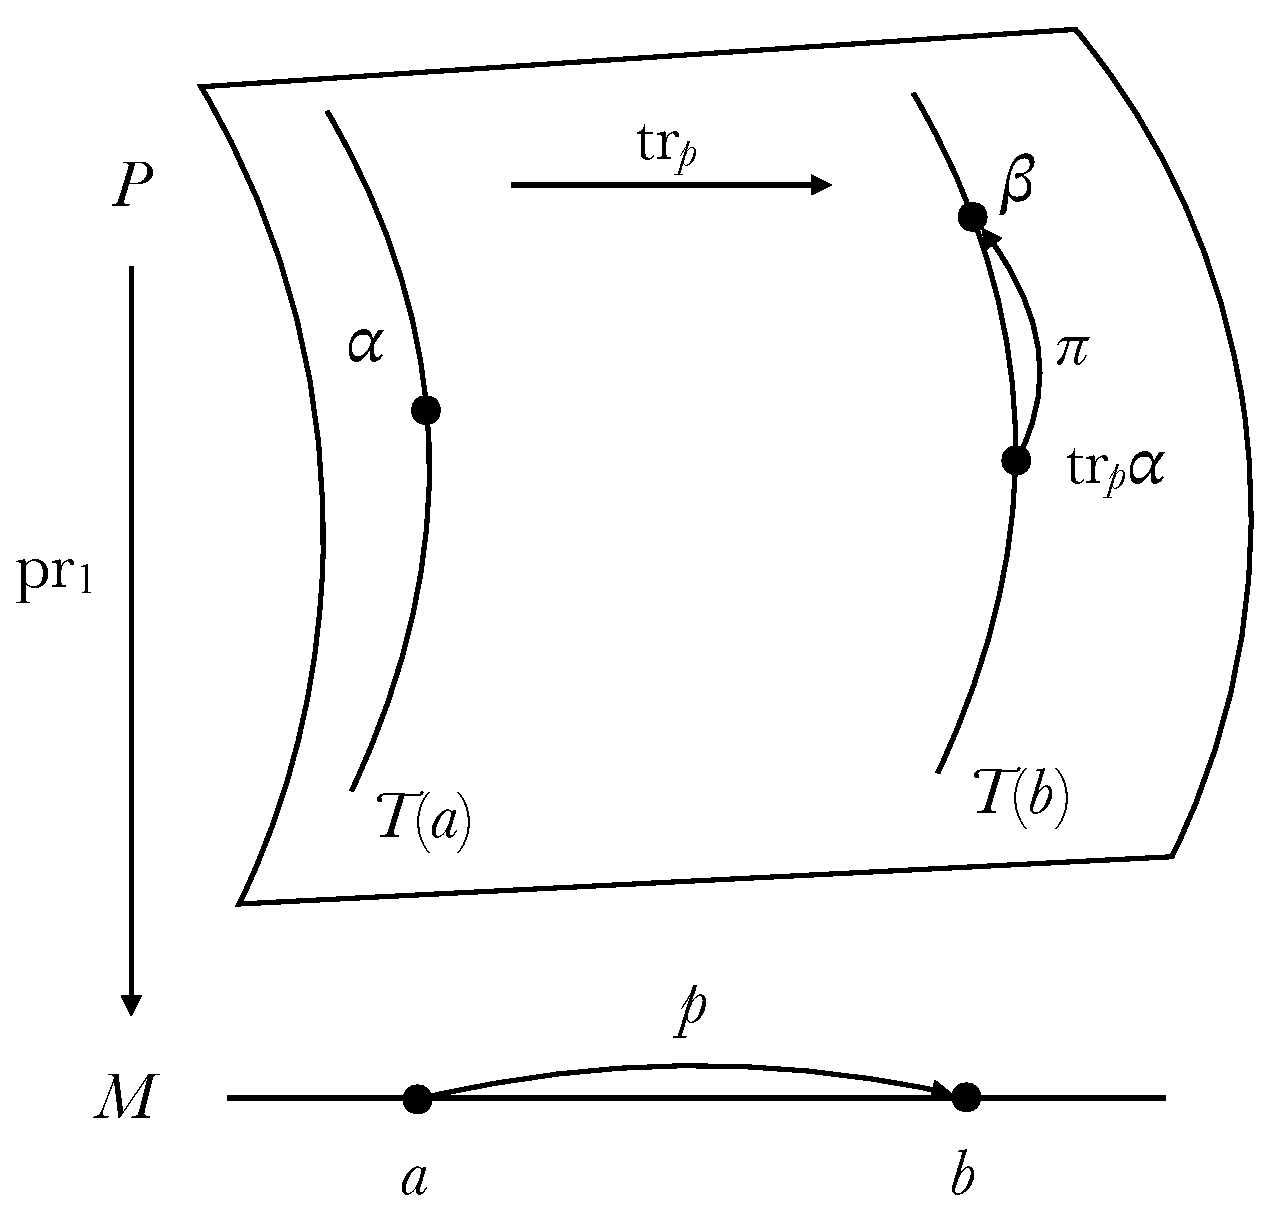
\includegraphics[width=200pt]{figs/pathovers.pdf}
\caption{A path \( \pi \) over the path \( p \) in the base involves the transport function.}
\label{fig:pathovers}
\end{figure}

Lastly we want to recall that in the presence of a section \( X:M\to P \) there is a dependent generalization of \( \ap \) called \( \apd \): \( \apd(X)(p):\tr(p)(X(a))=X(b) \) which is a pathover between the two values of the section over the basepoints of the path \( p \).

\clearpage
\section{Discrete manifolds}
\label{sec:discrete_man}
We will remind ourselves of the definition of a classical simplicial complex, in sets. Then we will create a type that realizes the data of a complex, using pushouts.

\subsection{Abstract simplicial complexes}

\begin{mydef}
An \defemph{abstract simplicial complex \( M \) of dimension \( n \)} is an ordered list \( M\defeq[M_0,\ldots,M_n] \) consisting of a set \( M_0 \) of vertices, and for each \( 0<k\leq n \) a set \( M_k \) of subsets of \( M_0 \) of cardinality \( k+1 \), such that for any \( j<k \), any \( (j+1) \)-element subset of an element of \( M_k \) is an element of \( M_j \). The elements of \( M_k \) are called \defemph{\( k \)-faces}. A \defemph{morphism} \( f \) from \( M=[M_0,\ldots,M_m] \) to \( N=[N_0,\ldots,N_n] \) is a function on vertices \( f:M_0\to N_0 \) such that for any face of \( M \) the image under \( f \) is a face of \( N \). Denote by \( \simcomp \) the type of abstract simplicial complexes of dimension \( n \). Let \( M_{\leq k}\defeq [M_0,\ldots,M_k] \). We call \( M_{\leq k} \) the \defemph{\( k \)-skeleton} of \( M \), and it is a (\( k \)-)complex in its own right. \( M \) is automatically equipped with a chain of inclusions of the skeleta \( M_0\hookrightarrow M_{\leq 1}\hookrightarrow\cdots\hookrightarrow M_{\leq n}=M \), which are simply the inclusions of lists into longer lists.
\end{mydef}

We can imagine constructing a simplicial complex dimension by dimension with a simple procedure of taking unions. This will parallel the realization construction that follows.

\begin{mydef}
Denote by \( \Delta(n) \) the simplicial complex obtained by taking the set of all subsets of the standard \( (n+1) \)-element set \( \Delta(n)_0\defeq\{0,\ldots,n\} \). We call \( \Delta(n) \) the \defemph{complete \( n \)-simplex}. We will refer to the \( (n-1) \)-skeleton \( \Delta(n)_{\leq(n-1)} \) with the suggestive notation \( \partial \Delta(n) \).
\end{mydef}

Note that \( \Delta(n)_{(n-1)} \) has \( n+1 \) elements. For example, \( \Delta(2)_1 \) consists of the three 2-element subsets of \( \{0, 1, 2\} \). 

Given \( M=[M_0,\ldots,M_n] \) and \( k\leq n \), a face \( f_k:M_k \) is the union of \( (k+1) \) faces in \( M_{k-1} \), and so the \( k \)-skeleton is obtained from the \( (k-1) \)-skeleton by forming the following pushout of sets:
\begin{equation}
% https://q.uiver.app/#q=WzAsNCxbMSwwLCJNX2siXSxbMCwwLCJNX2tcXHRpbWVzXFxwYXJ0aWFsIFAoaykiXSxbMCwxLCJNX3tcXGxlcSAoay0xKX0iXSxbMSwxLCJNX3tcXGxlcSBrfSJdLFsxLDAsIlxcbWF0aHJte3ByfV8xIl0sWzEsMiwiYV9rIiwyXSxbMCwzXSxbMiwzXSxbMywxLCIiLDEseyJzdHlsZSI6eyJuYW1lIjoiY29ybmVyLWludmVyc2UifX1dXQ==
\begin{tikzcd}
  {M_k\times\partial \Delta(k)} & {M_k} \\
  {M_{\leq (k-1)}} & {M_{\leq k}}
  \arrow["{\mathrm{pr}_1}", from=1-1, to=1-2]
  \arrow["{a_k}"', from=1-1, to=2-1]
  \arrow[from=1-2, to=2-2]
  \arrow[from=2-1, to=2-2]
  \arrow["\ulcorner"{anchor=center, pos=0.125, rotate=180}, draw=none, from=2-2, to=1-1]
\end{tikzcd}
\label{eq:attach}
\end{equation}
where the vertical ``attach'' map \( a_k(f_k, -) \) picks out the \( k+1 \) subsets of \( f_k \).

\begin{mydef}
In an abstract simplicial complex \( M \) of dimension \( n \), the \defemph{link} of a vertex \( v \) is the \( (n-1) \)-dimensional subcomplex containing every face \( m\in M_{n-1} \) such that \( v\notin m \) and \( m\cup v \) is an \( n \)-face of \( M \).
\label{def:link}
\end{mydef}

The link is easier to understand as all the neighboring vertices of \( v \) and the subcomplex containing these. See for example Figure~\ref{fig:link}.

\begin{figure}[h]
\centering
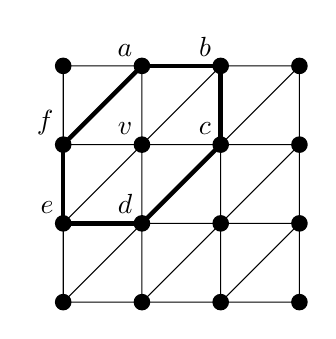
\begin{tikzpicture}
  \draw
    (0, 0) grid[step=1cm] (3, 3)
    (0, 2) edge[ultra thick] (1, 3)
    (0, 1) edge[ultra thick] (0, 2)
    (0, 1) edge[ultra thick] (1, 1)
    (1, 1) edge[ultra thick] (2, 2)
    (2, 2) edge[ultra thick] (2, 3)
    (1, 3) edge[ultra thick] (2, 3)
    (0, 1) -- (2, 3)
    (0, 0) -- (3, 3)
    (1, 0) -- (3, 2)
    (2, 0) -- (3, 1);
  \fill[radius=3pt]
    \foreach \x in {0, ..., 3} {
      \foreach \y in {0, ..., 3} {
        (\x, \y) circle[]
    }};
  \path[above left]
    \foreach \p/\v in {
      {1, 3}/a,
      {2, 3}/b,
      {0, 2}/f,
      {1, 2}/v,
      {2, 2}/c,
      {0, 1}/e,
      {1, 1}/d%
    } {
      (\p) node {$\v$}
    };
\end{tikzpicture}

\caption{The link of \( v \) in this complex consists of the vertices \( \{a,b,c,d,e,f\} \) and the edges \( \{ab,bc,cd,de,ef,fa\} \), forming a hexagon.}
\label{fig:link}
\end{figure}

\begin{mynote}
The \emph{geometric realization} of a complex uses the combinatorial data to form pushouts of standard simplices inside the category of topological spaces. A \emph{simplicial sphere} is a simplicial complex whose geometric realization is homeomorphic to a sphere. A classical 1940 result of Whitehead, building on Cairn, states that every smooth \( n \)-manifold is the geometric realization of a simplicial complex of dimension \( n \) such that the link is the geometric realization of an \( (n-1) \)-sphere\cite{whitehead_triangulation}. For more of this theory see the classic book by Kirby and Siebenmann\cite{kirby_siebenmann}.
\end{mynote}

\subsection{Higher inductive realizations}

We will realize a simplicial complex as a higher inductive type by forming a sequence of pushouts. We will work upward by dimension so as to define a standard sphere that we need in the next dimension.

\begin{mydef}
The \defemph{realization \( \mm \) of a 0-dimensional simplicial complex} \( M \) is simply the set \( M_0 \).
\end{mydef}

\begin{mydef}
The \defemph{simplicial 0-sphere} \( \bdsimplexn{1} \) is the realization of \( \partial \Delta(1) \).
\end{mydef}

\begin{mydef}
The \defemph{realization \( \mm \) of a 1-dimensional simplicial complex} \( M=[M_0, M_1] \) is the pushout
\end{mydef}
\begin{center}
% https://q.uiver.app/#q=WzAsNCxbMCwxLCJNXzA9XFxtYXRoYmJ7TX1fMCJdLFsxLDEsIlxcbWF0aGJie019XzEiXSxbMSwwLCJNXzEiXSxbMCwwLCJNXzFcXHRpbWVzIFxcYmRzaW1wbGV4bnsxfSJdLFswLDFdLFszLDAsIlxcbWF0aGJie0F9XzAiLDJdLFszLDIsIlxcbWF0aHJte3ByfV8xIl0sWzIsMSwiKl97XFxtYXRoYmJ7TX1fMX0iXSxbMSwzLCIiLDIseyJvZmZzZXQiOjMsInN0eWxlIjp7Im5hbWUiOiJjb3JuZXItaW52ZXJzZSJ9fV0sWzAsMiwiaF8xIiwyLHsic2hvcnRlbiI6eyJzb3VyY2UiOjQwLCJ0YXJnZXQiOjQwfSwibGV2ZWwiOjJ9XV0=
\begin{tikzcd}
  {M_1\times \bdsimplexn{1}} & {M_1} \\
  {M_0=\mathbb{M}_0} & {\mathbb{M}_1}
  \arrow["{\mathrm{pr}_1}", from=1-1, to=1-2]
  \arrow["{\mathbb{A}_0}"', from=1-1, to=2-1]
  \arrow["{*_{\mathbb{M}_1}}", from=1-2, to=2-2]
  \arrow["{h_1}"', shorten <=14pt, shorten >=14pt, Rightarrow, from=2-1, to=1-2]
  \arrow[from=2-1, to=2-2]
  \arrow["\ulcorner"{pos=0, rotate=180}, shift left=1, draw=none, from=2-2, to=1-1]
\end{tikzcd}
\end{center}
where \( a_k \) is the attachment data of the edges in \( M_1 \), as in diagram~\ref{eq:attach}. The right vertical map \( *_{\mm_1} \) provides a hub point for each edge, and the homotopy \( h_1 \) provides the spokes that connect the hub to the vertices.

\begin{mydef}
The \defemph{simplicial 1-sphere} \( \bdsimplexn{2} \) is the realization of \( \partial \Delta(2) \).
\end{mydef}
\begin{center}% https://q.uiver.app/#q=WzAsNCxbMCwxLCJQKDIpXzAiXSxbMSwxLCJcXHBhcnRpYWwgXFxEZWx0YV4yIl0sWzEsMCwiXFxwYXJ0aWFsIFAoMikiXSxbMCwwLCJcXHBhcnRpYWwgUCgyKVxcdGltZXMgXFxwYXJ0aWFsIFxcRGVsdGFeMSJdLFswLDFdLFszLDAsIlxcbWF0aGJie0F9XzAiLDJdLFszLDIsIlxcbWF0aHJte3ByfV8xIl0sWzIsMSwiKl97XFxwYXJ0aWFsXFxEZWx0YV4yfSJdLFsxLDMsIiIsMix7InN0eWxlIjp7Im5hbWUiOiJjb3JuZXItaW52ZXJzZSJ9fV0sWzAsMiwiaF8xIiwyLHsic2hvcnRlbiI6eyJzb3VyY2UiOjQwLCJ0YXJnZXQiOjQwfSwibGV2ZWwiOjJ9XV0=
\begin{tikzcd}
  {\partial \Delta(2)\times \bdsimplexn{1}} & {\partial \Delta(2)} \\
  {\Delta(2)_0} & {\bdsimplex{2}}
  \arrow["{\mathrm{pr}_1}", from=1-1, to=1-2]
  \arrow["{\mathbb{A}_0}"', from=1-1, to=2-1]
  \arrow["{*_{\bdsimplexn{2}}}", from=1-2, to=2-2]
  \arrow["{h_1}"', shorten <=11pt, shorten >=11pt, Rightarrow, from=2-1, to=1-2]
  \arrow[from=2-1, to=2-2]
  \arrow["\ulcorner"{anchor=center, pos=0.125, rotate=180}, draw=none, from=2-2, to=1-1]
\end{tikzcd}
\end{center}

\begin{mydef}
A \defemph{realization \( \mm \) of a 2-dimensional simplicial complex} \( [M_0, M_1, M_2] \) is the pushout
\end{mydef}
\begin{center}
% https://q.uiver.app/#q=WzAsNyxbMCwyLCJNXzFcXHRpbWVzIFxcYmRzaW1wbGV4bnsxfSJdLFswLDEsIlxcbWF0aGJie019XzAiXSxbMSwxLCJcXG1hdGhiYntNfV8xIl0sWzEsMiwiTV8xIl0sWzEsMCwiTV8yXFx0aW1lcyBcXGJkc2ltcGxleG57Mn0iXSxbMiwwLCJNXzIiXSxbMiwxLCJcXG1hdGhiYntNfV8yIl0sWzAsMSwiXFxtYXRoYmJ7QX1fMCJdLFsxLDJdLFswLDMsIlxcbWF0aHJte3ByfV8xIiwyXSxbMywyLCIqX3tcXG1hdGhiYntNfV8xfSIsMl0sWzIsMCwiIiwxLHsic3R5bGUiOnsibmFtZSI6ImNvcm5lci1pbnZlcnNlIn19XSxbMiw2XSxbNCwyLCJcXG1hdGhiYntBfV8xIiwyXSxbNSw2LCIqX3tcXG1hdGhiYntNfV8yfSJdLFs0LDUsIlxcbWF0aHJte3ByfV8xIl0sWzYsNCwiIiwxLHsic3R5bGUiOnsibmFtZSI6ImNvcm5lci1pbnZlcnNlIn19XSxbMiw1LCJoXzIiLDAseyJzaG9ydGVuIjp7InNvdXJjZSI6NDAsInRhcmdldCI6NDB9LCJsZXZlbCI6Mn1dLFsxLDMsImhfMSIsMix7InNob3J0ZW4iOnsic291cmNlIjo0MCwidGFyZ2V0Ijo0MH0sImxldmVsIjoyfV1d
\begin{tikzcd}
  & {M_2\times \bdsimplexn{2}} & {M_2} \\
  {\mathbb{M}_0} & {\mathbb{M}_1} & {\mathbb{M}_2} \\
  {M_1\times \bdsimplexn{1}} & {M_1}
  \arrow["{\mathrm{pr}_1}", from=1-2, to=1-3]
  \arrow["{\mathbb{A}_1}"', from=1-2, to=2-2]
  \arrow["{*_{\mathbb{M}_2}}", from=1-3, to=2-3]
  \arrow[from=2-1, to=2-2]
  \arrow["{h_1}"', shorten <=27pt, shorten >=27pt, Rightarrow, from=2-1, to=3-2]
  \arrow["{h_2}", shorten <=17pt, shorten >=17pt, Rightarrow, from=2-2, to=1-3]
  \arrow[from=2-2, to=2-3]
  \arrow["\ulcorner"{anchor=center, pos=0.125, rotate=-135}, draw=none, from=2-2, to=3-1]
  \arrow["\ulcorner"{anchor=center, pos=0.125, rotate=180}, draw=none, from=2-3, to=1-2]
  \arrow["{\mathbb{A}_0}", from=3-1, to=2-1]
  \arrow["{\mathrm{pr}_1}"', from=3-1, to=3-2]
  \arrow["{*_{\mathbb{M}_1}}"', from=3-2, to=2-2]
\end{tikzcd}

\end{center}
where \( \aaa_1 \) is such that this additional diagram commutes
\begin{center}
% https://q.uiver.app/#q=WzAsNCxbMSwwLCJNXzJcXHRpbWVzXFxwYXJ0aWFsXFxEZWx0YV4yIl0sWzEsMSwiXFxtYXRoYmJ7TX1fMSJdLFswLDAsIk1fMlxcdGltZXNcXHBhcnRpYWwgUCgyKSJdLFswLDEsIk1fe1xcbGVxIDF9Il0sWzAsMSwiXFxtYXRoYmJ7QX1fMSJdLFsyLDAsIlxcbWF0aHJte2lkfVxcdGltZXMgKl97XFxwYXJ0aWFsXFxEZWx0YV4yfSJdLFszLDEsIipfe1xcbWF0aGJie019X3tcXGxlcSAxfX0iLDJdLFsyLDMsImFfMSIsMl1d
\begin{tikzcd}
  {M_2\times\partial \Delta(2)} & {M_2\times\bdsimplexn{2}} \\
  {M_{\leq 1}} & {\mathbb{M}_1}
  \arrow["{\mathrm{id}\times *_{\bdsimplexn{2}}}", from=1-1, to=1-2]
  \arrow["{a_1}"', from=1-1, to=2-1]
  \arrow["{\mathbb{A}_1}", from=1-2, to=2-2]
  \arrow["{*_{\mathbb{M}_{\leq 1}}}"', from=2-1, to=2-2]
\end{tikzcd}
\end{center}
In this diagram \( a_1 \) is the simplicial attaching map from \ref{eq:attach}, and \( *_{\mathbb{M}_{\leq 1}} \) simply gathers the hub maps from \( M_0 \) and \( M_1 \) into \( \mm_1 \). The commutativity then says that \( \aaa_1 \) reflects the attachment data.
\begin{mydef}
Given a notion of realization in dimension \( n-1 \), a \defemph{realization \( \mm \) of an \( n \)-dimensional simplicial complex} \( M=[M_0, \ldots, M_n] \) is the pushout
\end{mydef}
\begin{center}%
% https://q.uiver.app/#q=WzAsMTAsWzIsMSwiXFxtYXRoYmJ7TX1fe24tMX0iXSxbMiwwLCJNX25cXHRpbWVzIFxccGFydGlhbFxcRGVsdGFebiJdLFszLDAsIk1fbiJdLFszLDEsIlxcbWF0aGJie019X24iXSxbMSwxLCJcXG1hdGhiYntNfV97bi0yfSJdLFsxLDAsIk1fe24tMn0iXSxbMiwyLCJNX3tuLTF9Il0sWzEsMiwiXFxjZG90cyJdLFswLDAsIlxcY2RvdHMiXSxbMCwxLCJcXGNkb3RzIl0sWzAsM10sWzEsMCwiXFxtYXRoYmJ7QX1fe24tMX0iLDJdLFsyLDMsIipfe1xcbWF0aGJie019X3tufX0iXSxbMSwyLCJcXG1hdGhybXtwcn1fMSJdLFszLDEsIiIsMSx7InN0eWxlIjp7Im5hbWUiOiJjb3JuZXItaW52ZXJzZSJ9fV0sWzAsMiwiaF9uIiwwLHsic2hvcnRlbiI6eyJzb3VyY2UiOjQwLCJ0YXJnZXQiOjQwfSwibGV2ZWwiOjJ9XSxbNCwwXSxbNSw0LCIqX3tcXG1hdGhiYntNfV97bi0yfX0iXSxbNiwwLCIqX3tcXG1hdGhiYntNfV97bi0xfX0iLDJdLFs4LDVdLFs5LDRdLFs3LDZdLFswLDcsIiIsMix7InN0eWxlIjp7Im5hbWUiOiJjb3JuZXItaW52ZXJzZSJ9fV0sWzQsOCwiIiwyLHsic3R5bGUiOnsibmFtZSI6ImNvcm5lci1pbnZlcnNlIn19XSxbOSw1LCJoX3tuLTJ9IiwwLHsic2hvcnRlbiI6eyJzb3VyY2UiOjQwLCJ0YXJnZXQiOjQwfSwibGV2ZWwiOjJ9XSxbNCw2LCJoX3tuLTF9IiwyLHsic2hvcnRlbiI6eyJzb3VyY2UiOjQwLCJ0YXJnZXQiOjQwfSwibGV2ZWwiOjJ9XV0=
\begin{tikzcd}
  \cdots & {M_{n-2}} & {M_n\times \bdsimplexn{n}} & {M_n} \\
  \cdots & {\mathbb{M}_{n-2}} & {\mathbb{M}_{n-1}} & {\mathbb{M}_n} \\
  & \cdots & {M_{n-1}}
  \arrow[from=1-1, to=1-2]
  \arrow["{*_{\mathbb{M}_{n-2}}}", from=1-2, to=2-2]
  \arrow["{\mathrm{pr}_1}", from=1-3, to=1-4]
  \arrow["{\mathbb{A}_{n-1}}"', from=1-3, to=2-3]
  \arrow["{*_{\mathbb{M}_{n}}}", from=1-4, to=2-4]
  \arrow["{h_{n-2}}", shorten <=8pt, shorten >=8pt, Rightarrow, from=2-1, to=1-2]
  \arrow[from=2-1, to=2-2]
  \arrow["\ulcorner"{anchor=center, pos=0.125, rotate=180}, draw=none, from=2-2, to=1-1]
  \arrow[from=2-2, to=2-3]
  \arrow["{h_{n-1}}"', shorten <=10pt, shorten >=10pt, Rightarrow, from=2-2, to=3-3]
  \arrow["{h_n}", shorten <=10pt, shorten >=10pt, Rightarrow, from=2-3, to=1-4]
  \arrow[from=2-3, to=2-4]
  \arrow["\ulcorner"{anchor=center, pos=0.125, rotate=-90}, draw=none, from=2-3, to=3-2]
  \arrow["\ulcorner"{anchor=center, pos=0.125, rotate=180}, draw=none, from=2-4, to=1-3]
  \arrow[from=3-2, to=3-3]
  \arrow["{*_{\mathbb{M}_{n-1}}}"', from=3-3, to=2-3]
\end{tikzcd}
\end{center}
where \( \aaa_n \) is such that the following commutes
\begin{center}
% https://q.uiver.app/#q=WzAsNCxbMSwwLCJNX25cXHRpbWVzXFxwYXJ0aWFsXFxEZWx0YV5uIl0sWzEsMSwiXFxtYXRoYmJ7TX1fbiJdLFswLDAsIk1fblxcdGltZXNcXHBhcnRpYWwgUChuKSJdLFswLDEsIk1fe1xcbGVxIG59Il0sWzAsMSwiXFxtYXRoYmJ7QX1fbiJdLFsyLDAsIlxcbWF0aHJte2lkfVxcdGltZXMgKl97XFxwYXJ0aWFsXFxEZWx0YV5ufSJdLFszLDEsIipfe1xcbWF0aGJie019X3tcXGxlcSBufX0iLDJdLFsyLDMsImFfMSIsMl1d
\begin{tikzcd}
  {M_n\times\partial \Delta(n)} & {M_n\times\bdsimplexn{n}} \\
  {M_{\leq n}} & {\mathbb{M}_n}
  \arrow["{\mathrm{id}\times *_{\bdsimplexn{n}}}", from=1-1, to=1-2]
  \arrow["{a_1}"', from=1-1, to=2-1]
  \arrow["{\mathbb{A}_n}", from=1-2, to=2-2]
  \arrow["{*_{\mathbb{M}_{\leq n}}}"', from=2-1, to=2-2]
\end{tikzcd}
\end{center}
Gathering some of the inductive process into one definition, we have
\begin{mydef}
\label{def:higher_realization} 
A \defemph{realization} \( \mm \) of an abstract simplicial complex \( M:\simcomp \) consists of 
\begin{enumerate}
\item \( n+1 \) types \( \mm_0,\ldots,\mm_n \) where \( \mm_0\defeq M_0 \),
\item \( n \) spans \( \myspan{\mm_{i}}{M_{i+1}\times \bdsimplexn{i+1}}{M_{i+1}}{\aaa_{i}}{\pr_1} \), \( i=0,\ldots,n-1 \), where \( \bdsimplexn{i+1} \) is the realization of the boundary of a standard simplex and \( \aaa_i \) are called \defemph{attachment maps},
\item \( n \) pushout squares from each span to \( \mm_{i+1} \), with induced maps \( \imath_i:\mm_i\to\mm_{i+1} \), \( *_{\mm_{i+1}}:M_{i+1}\to\mm_{i+1} \) and proof of commutativity \( h_{i+1} \).
\end{enumerate}
A \defemph{cellular type} \( \mm \) is a sequence of types \( \mm_0\xrightarrow[]{\imath_0}\mm_1\xrightarrow[]{\imath_1}\cdots\xrightarrow[]{\imath_{n-1}}\mm_n \), together with a proof of existence of some simplicial complex \( M \) and a realization inducing this sequence.
\end{mydef}

\subsection{Polygons}
\label{sec:polygons}

The 1-type \( \bdsimplexn{2} \) has three vertices. In order to define the link of an arbitrary realization, we will need to have \( n \)-gons for \( n\geq 3 \). For example in Figure~\ref{fig:link} the link is a 6-gon. And since \( S^1 \) could be called a 1-gon, we will also define a 1-gon, and for completeness a 2-gon.

\begin{mydef}
Define \( C(n) \), \( n\geq 3 \) to be a simplicial complex with \( C(n)_{0}=\{v_1, \ldots, v_n\} \) and edges \[ C(n)_1=\{e_1=\{v_1,v_2\}, \ldots, e_{n-1}=\{v_{n-1}, v_n\}, e_n=\{v_n, v_0\}\}. \] We call \( C(n) \) a \defemph{polygon} or \defemph{\( n \)-gon}. The realization of \( C(n) \) will be denoted \( \ccc(n) \). When it is convenient we may refer to an \( n \)-gon by \( \gr{v_1\cdots v_n} \) and to its realization by \( \hgr{v_1\cdots v_n} \).
\end{mydef}

We also have two special polygons:
\begin{mydef}
The higher inductive type \( \so \), also denoted \( \ccc(1) \), has constructors:
\begin{align*}
\so &:\Type \\
\mathsf{base}&:\so \\
\mathsf{loop}&:\mathsf{base}=\mathsf{base}
\end{align*}
\end{mydef}

\begin{mydef}
The higher inductive type \(\ccc(2) \) has constructors:
\begin{align*}
\ccc(2) &:\Type \\
v_1, v_2&:\ccc(2) \\
\ell_{12}, r_{21}&:v_1=v_2\\
\end{align*}
\end{mydef}

\begin{mylemma}\label{lem:addpoints}
\( \ccc(2)\simeq \ccc(1) \) and in fact \( \ccc(n)\simeq \ccc(n-1) \).
\end{mylemma}
\begin{myproofnonqed}
(Compare to \cite{hottbook} Lemma 6.5.1.)
\end{myproofnonqed}
First we will define \( f:\ccc(2)\to \ccc(1) \) and \( g:\ccc(1)\to \ccc(2) \), then prove they are inverses.
\begin{align*}
f(v_1)=f(v_2)&=\base &\quad g(\base)&=v_1\\
f(\ell_{12})&=\loopo&\quad g(\loopo)&=\ell_{12}\cdot r_{21}\\
f(r_{21}) &= \refl_{\base}& & \\
\end{align*}

We need to show that \( f\circ g\sim \id_{\ccc(1)} \) and \( g\circ f\sim\id_{\ccc(2)} \).
Think of \( f \) as sliding \( v_2 \) and \( v_1 \) towards each other along \( r_{21} \) coalescing into just \( v_1 \), as in Figure~\ref{fig:shrink}. This may help understand why the somewhat intricate proof is working.

\begin{figure}[h]
\centering
\begin{tikzpicture}
\tikzset{arrow/.style={-{Stealth[scale=1.1]}}}
\tikzset{oo/.style={circle, scale=0.25, fill=black}}
\tikzset{ooo/.style={circle, scale=0.25, fill=none}}
\node[oo, label=above:\( v_1 \)] (V1) at (0, 2) {};
\node[oo, label=below:\( v_2 \)] (V2) at (0, 0) {};
\node[ooo] (V21) at (0.3, 1.75) {};
\node[ooo] (V22) at (0.3, 0.25) {};
\draw (V1) edge[bend right=60, swap, "\( \ell_{12} \)"] (V2);
\draw (V1) edge[bend left=60, "\( r_{21} \)"] (V2);
\draw[arrow] (V1) edge[bend left=5] (V21);
\draw[arrow] (V2) edge[bend right=5] (V22);
\end{tikzpicture}
\caption{We imagine shrinking \( r_{21} \) down to become \( \refl_\base \) in \( S^1 \).}
\label{fig:shrink}
\end{figure}

We need terms \( p:\pit{a:\ccc(1)}f(g(a))=a \) and \( q:\pit{a:\ccc(2)}g(f(a))=a \). We will proceed by induction, defining appropriate paths on point constructors and then checking a condition on path constructors that confirms that the built-in transport of these type families respects the definition on points.

Looking first at \( g\circ f \), which shrinks \( r_{21} \), we have the following data to work with:
\begin{align*}
g(f(v_1))=g(f(v_2))&=v_1\\
g(f(\ell_{12}))&=\ell_{12}\cdot r_{21}\\
g(f(r_{21})) &= \refl_{v_1}.
\end{align*}
We then need to supply a homotopy from this data to \( \id_{\ccc(2)} \), which consists of a section and pathovers over \( \ccc(2) \):
\begin{align*}
p_1&:g(f(v_1))=v_1\\
p_2&:g(f(v_1))=v_2\\
H_\ell&:\tr(\ell_{12})(p_1)=p_2\\
H_r&:\tr(r_{21})(p_2)=p_1.
\end{align*}
which simplifies to
\begin{align*}
p_1&:v_1=v_1\\
p_2&:v_1=v_2\\
H_\ell&:g(f(\ell_{12}))^{-1}\cdot p_1\cdot \ell_{12}=p_2\\
H_r&:=g(f(r_{21}))^{-1}\cdot p_2\cdot r_{21}= p_1
\end{align*}
and then to 
\begin{align*}
p_1&:v_1=v_1\\
p_2&:v_1=v_2\\
H_\ell&:(\ell_{12}\cdot r_{21})^{-1}\cdot p_1\cdot \ell_{12}=p_2\\
H_r&:\refl_{v_1}\cdot p_2\cdot r_{21}= p_1
\end{align*}

To solve all of these constraints we can choose \( p_1\defeq\refl_{v_1} \), which by consulting either \( H_\ell \) or \( H_r \) requires that we take \( p_2\defeq{r_{21}}^{-1}\).

Now examining \( f\circ g \), we have
\begin{align*}
f(g(\base))&=\base&\\
f(g(\loopo))&=f(\ell_{12}\cdot r_{21})=\loopo
\end{align*}
and so we have an easy proof that this is the identity.

The proof of the more general case \( \ccc(n) \simeq \ccc(n-1)\) is very similar. Take the maps \( f:\ccc(n)\to \ccc(n-1) \), \( g:\ccc(n-1)\to \ccc(n) \) to be
\begin{align*}
f(v_i)=v_i&\quad(i=1,\ldots,n-1) & g(v_i)&=v_i&\quad(i=1,\ldots,n-1)\\
f(v_n)=v_1&\quad& g(e_{i,i+1})&=e_{i,i+1}&\quad(i=1,\ldots,n-2)\\
f(e_{i,i+1})=e_{i,i+1}&\quad(i=1,\ldots,n-1)& g(e_{n-1,1})&=e_{n-1,n}\cdot e_{n,1}&\\
f(e_{n-1,n})=e_{n-1,1}&&&&\\
f(e_{n,1})=\refl_{v_1}&&&&
\end{align*}
where \( f \) should be thought of as shrinking \( e_{n,1} \) so that \( v_n \) coalesces into \( v_1 \).

The proof that \( g\circ f\sim\id_{\ccc(n)} \) proceeds as follows: the composition is definitionally the identity except 
\begin{align*}
g(f(v_n))&=v_1\\
g(f(e_{n-1,n}))&=e_{n-1,n}\cdot e_{n,1}\\
g(f(e_{n,1}))&= \refl_{v_1}.
\end{align*}
Guided by our previous experience we choose \( {e_{n,1}}^{-1}:g(f(v_n))=v_n \), and define the pathovers by transport.

The proof that \( f\circ g\sim\id_{\ccc(n-1)} \) requires only noting that \( f(g(e_{n-1,1}))=f(e_{n-1,n}\cdot e_{n,1})=e_{n-1,1}\cdot\refl_{v_1}=e_{n-1,1} \).\qed

\begin{mycor}
\label{cor:gon}
All polygons are equivalent to \( \so \), i.e. we have terms \( e_n:\ccc(n)=S^1 \), and hence we have constructed a map from the unit type \( (\ccc(n), ||e_n||_{-1}):\unit\to \EMzo \).
\end{mycor}
\begin{myproof}
The proofs in Lemma~\ref{lem:addpoints} can be concatenated to give \( \ccc(n)\to\ccc(n-1)\to\cdots\to\ccc(2)\to S^1 \).
\end{myproof}

\begin{mydef}
\label{def:rotation}
Let \( R:\gr{v_1\cdots v_n}\to \gr{v_1\cdots v_n} \) (for ``rotation'') be the map sending \( v_i\mapsto v_{i+1} \) and \( v_n\mapsto v_0 \). This map clearly sends edges to edges, and so is a map of simplicial complexes, and extends to a map \( \hgr{R}:\hgr{v_1\cdots v_n}\to \hgr{v_1\cdots v_n} \).
\end{mydef}

The homotopical realization \( \hgr{R} \) has a path to the identity:
\begin{mylemma}
\label{lem:rotation}
The map \( \hgr{R}: \hgr{v_1\cdots v_n}\to \hgr{v_1\cdots v_n}\) is connected to \( \refl_{\hgr{v_1\cdots v_n}} \) by a homotopy \( H_R:\pit{x:\hgr{v_1\cdots v_n}}x=\hgr{R}(x) \).
\end{mylemma}
\begin{myproof}
If \( x \) is a vertex, take \( H_R(x) \) to be the obvious unique edge back to the starting vertex. This extends in the obvious functorial way to edges.
\end{myproof}

We wrote the homotopy \( H_R(x) \) as starting at \( x \) because it feels like a record of a time-based process of applying \( R \). We will rely on this convention when we define flatness.

\subsection{Surfaces}
We will eventually focus on 2-dimensional simplicial complexes in this note, and our running example which begins in the next section is 2-dimensional. We have a simple way to define an orientation in this dimension, which we provide here. We will touch on the relationship between this classical definition and the definition of our HoTT classifying space when we discuss vector fields in Section~\ref{sec:vector_field_def}.

\begin{mydef}
An \defemph{orientation} \( \mathscr{O} \) of a 2-dimensional simplicial complex \( M=[M_0, M_1, M_2] \) is an equivalence class of ordering maps \( V:M_2\to \mathsf{List} \) to the type of ordered lists, where \( V \) orders the vertices of every 2-face. If \( F:M_2 \) is a face and \( F=\{a, b, c\} \) are its vertices, then \( V(F) \) is a list of all the vertices, e.g. \( [b, c, a] \). Two orderings \( V, V' \) are said to have the \defemph{same orientation} if it is true for every face \( F \) that \( V(F) \) and \( V'(F) \) differ by a cyclic permutation. The inclusion \( e\subset F \) of an edge in a face induces an ordering of the vertices of the edge, called \defemph{the induced order of \( e\subset F \)}.
\end{mydef}

\subsection{The octahedron model of the sphere}
We will create our first combinatorial surface, an octahedron. In \( \simcomp \) the combinatorial data of the faces can be represented with a \emph{Hasse diagram}, which shows the poset of inclusions in a graded manner, with a special top and bottom element. The top element is part of the diagram only, and not part of the simplicial complex, else it would provide a filling cell. We give an octahedron \( O=[O_0, O_1, O_2] \) in Figure~\ref{fig:hasse_octohedron}. The names of the vertices are short for white, yellow, blue, red, green, and orange, the colors of the faces of a Rubik's cube. The octahedron is the dual of the cube, with each vertex corresponding to a face.

\begin{figure}[h]
\centering
\begin{tikzpicture}
    \matrix (A) [matrix of math nodes, row sep=1cm, column sep=-.2cm]
    { 
       ~ &  ~ & ~ & ~ & ~ & \left\{\substack{{w, b, r}\\ {g, o, y}}\right\} \\  
  ~ &  ~ & \scriptstyle\{w, b, r\} & \scriptstyle\{w, r, g\}  & \scriptstyle\{w, g, o\} & \scriptstyle\{w, o, b\} & \scriptstyle\{y, b, r\} & \scriptstyle\{y, r, g\}  & \scriptstyle\{y, g, o\} & \scriptstyle\{y, o, b\}\\
  \scriptstyle\{w, b\} & \scriptstyle\{w,r\}  & \scriptstyle\{w,g\} & \scriptstyle\{w,o\} & \scriptstyle\{b, r\} & \scriptstyle\{r, g\}  & \scriptstyle\{g, o\} & \scriptstyle\{o, b\} & \scriptstyle\{y, b\} & \scriptstyle\{y,r\}  & \scriptstyle\{y,g\} & \scriptstyle\{y,o\}\\
  ~ & ~ & ~ &  \scriptstyle\{w\}  & \scriptstyle\{b\} & \scriptstyle\{r\} & \scriptstyle\{g\} & \scriptstyle\{o\} & \scriptstyle\{y\}\\
      ~ & ~ &  ~ & ~ & ~ & \emptyset \\
    };
    \draw (A-1-6.south)--(A-2-3.north);
    \draw (A-1-6.south)--(A-2-4.north);
    \draw (A-1-6.south)--(A-2-5.north);
    \draw (A-1-6.south)--(A-2-6.north);
    \draw (A-1-6.south)--(A-2-7.north);
    \draw (A-1-6.south)--(A-2-8.north);
    \draw (A-1-6.south)--(A-2-9.north);
    \draw (A-1-6.south)--(A-2-10.north);

    \draw (A-2-3.south)--(A-3-1.north);
    \draw (A-2-3.south)--(A-3-2.north);
    \draw (A-2-3.south)--(A-3-5.north);

    \draw (A-2-4.south)--(A-3-2.north);
    \draw (A-2-4.south)--(A-3-3.north);
    \draw (A-2-4.south)--(A-3-6.north);

    \draw (A-2-5.south)--(A-3-3.north);
    \draw (A-2-5.south)--(A-3-4.north);
    \draw (A-2-5.south)--(A-3-7.north);

    \draw (A-2-6.south)--(A-3-4.north);
    \draw (A-2-6.south)--(A-3-1.north);
    \draw (A-2-6.south)--(A-3-8.north);

    \draw (A-2-7.south)--(A-3-5.north);
    \draw (A-2-7.south)--(A-3-10.north);
    \draw (A-2-7.south)--(A-3-9.north);

    \draw (A-2-8.south)--(A-3-6.north);
    \draw (A-2-8.south)--(A-3-11.north);
    \draw (A-2-8.south)--(A-3-10.north);

    \draw (A-2-9.south)--(A-3-7.north);
    \draw (A-2-9.south)--(A-3-12.north);
    \draw (A-2-9.south)--(A-3-11.north);

    \draw (A-2-10.south)--(A-3-8.north);
    \draw (A-2-10.south)--(A-3-9.north);
    \draw (A-2-10.south)--(A-3-12.north);

    \draw (A-3-1.south)--(A-4-4.north);
    \draw (A-3-1.south)--(A-4-5.north);

    \draw (A-3-2.south)--(A-4-4.north);
    \draw (A-3-2.south)--(A-4-6.north);

    \draw (A-3-3.south)--(A-4-4.north);
    \draw (A-3-3.south)--(A-4-7.north);

    \draw (A-3-4.south)--(A-4-4.north);
    \draw (A-3-4.south)--(A-4-8.north);

    \draw (A-3-5.south)--(A-4-5.north);
    \draw (A-3-5.south)--(A-4-6.north);

    \draw (A-3-6.south)--(A-4-6.north);
    \draw (A-3-6.south)--(A-4-7.north);

    \draw (A-3-7.south)--(A-4-7.north);
    \draw (A-3-7.south)--(A-4-8.north);

    \draw (A-3-8.south)--(A-4-8.north);
    \draw (A-3-8.south)--(A-4-5.north);

    \draw (A-3-9.south)--(A-4-9.north);
    \draw (A-3-9.south)--(A-4-5.north);

    \draw (A-3-10.south)--(A-4-9.north);
    \draw (A-3-10.south)--(A-4-6.north);

    \draw (A-3-11.south)--(A-4-9.north);
    \draw (A-3-11.south)--(A-4-7.north);

    \draw (A-3-12.south)--(A-4-9.north);
    \draw (A-3-12.south)--(A-4-8.north);

    \draw (A-4-4.south)--(A-5-6.north);
    \draw (A-4-5.south)--(A-5-6.north);
    \draw (A-4-6.south)--(A-5-6.north);
    \draw (A-4-7.south)--(A-5-6.north);
    \draw (A-4-8.south)--(A-5-6.north);
    \draw (A-4-9.south)--(A-5-6.north);

\end{tikzpicture}
\begin{figure}[h]
\centering
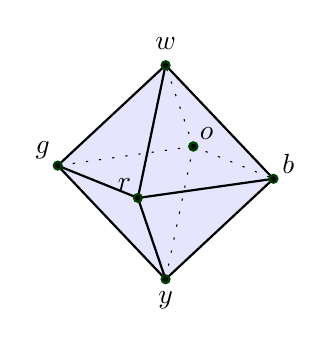
\begin{tikzpicture}%
  [x={(-0.860769cm, -0.121512cm)},
  y={(0.508996cm, -0.205391cm)},
  z={(-0.000053cm, 0.971107cm)},
  scale=1,
  back/.style={loosely dotted, thin},
  edge/.style={black, thick},
  facet/.style={fill=blue!95!black,fill opacity=0.1},
  vertex/.style={inner sep=1pt,circle,draw=green!25!black,fill=black,thick}]
\coordinate (-1, -1, 0) at (-1, -1, 0);
\coordinate (-1, 1, 0) at (-1, 1, 0);
\coordinate (0, 0, -1) at (0, 0, -1);
\coordinate (0, 0, 1) at (0, 0, 1);
\coordinate (1, -1, 0) at (1, -1, 0);
\coordinate (1, 1, 0) at (1, 1, 0);
%% Drawing edges in the back
%%
\draw[edge,back] (-1, -1, 0) -- (-1, 1, 0);
\draw[edge,back] (-1, -1, 0) -- (0, 0, -1.4);
\draw[edge,back] (-1, -1, 0) -- (0, 0, 1.4);
\draw[edge,back] (-1, -1, 0) -- (1, -1, 0);
%% Drawing vertices in the back
%%
\node[vertex] at (-1, -1, 0)     {};
%% Drawing the facets
%%
\fill[facet] (1, 1, 0) -- (0, 0, -1.4) -- (1, -1, 0) -- cycle {};
\fill[facet] (1, 1, 0) -- (0, 0, 1.4) -- (1, -1, 0) -- cycle {};
\fill[facet] (1, 1, 0) -- (-1, 1, 0) -- (0, 0, 1.4) -- cycle {};
\fill[facet] (1, 1, 0) -- (-1, 1, 0) -- (0, 0, -1.4) -- cycle {};
%% Drawing edges in the front
%%
\draw[edge] (-1, 1, 0) -- (0, 0, -1.4);
\draw[edge] (-1, 1, 0) -- (0, 0, 1.4);
\draw[edge] (-1, 1, 0) -- (1, 1, 0);
\draw[edge] (0, 0, -1.4) -- (1, -1, 0);
\draw[edge] (0, 0, -1.4) -- (1, 1, 0);
\draw[edge] (0, 0, 1.4) -- (1, -1, 0);
\draw[edge] (0, 0, 1.4) -- (1, 1, 0);
\draw[edge] (1, -1, 0) -- (1, 1, 0);
%% Drawing the vertices in the front
%%
\begin{scope}[nodes=vertex]
\node[label=above right:\( b \)] at (-1, 1, 0)     {};
\node[label=below:\( y \)] at (0, 0, -1.4)     {};
\node[label=above:\( w \)] at (0, 0, 1.4)     {};
\node[label=above left:\( g \)] at (1, -1, 0)     {};
\node[label=above left:\( r \)] at (1, 1, 0)     {};
\node[label=above right:\( o \)] at (-1, -1, 0)     {};
\end{scope}
\end{tikzpicture}
\caption{The HIT \( \oo \) which has 6 points, 12 1-paths, 8 2-paths.}
\end{figure}

\caption{The Hasse diagram of the simplicial complex \( O \), and a possible realization. The row of singletons in the Hasse diagram is \( O_0 \) and above it are \( O_1 \) and \( O_2 \).}
\label{fig:hasse_octohedron}
\end{figure}

We can realize \( O=[O_0, O_1, O_2] \) as a cellular type \( \oo \).

\begin{mylemma}
\label{lem:octahedron_sphere}
There is an equivalence \( \oo_2\simeq S^2 \).
\end{mylemma}
\begin{myproof}Omitted.\end{myproof}

\clearpage
\section{Bundles, connections, and curvature}
A map out of a higher combinatorial manifold has various components. These line up with classical definitions, and identifying those is a primary purpose of this note.

\subsection{Definitions}

\begin{mydef}
\label{def:connection}
If \( \mm \) is a higher combinatorial \( n \)-manifold and \( f_k:\mm_k\to\uni \) are type families on each skeleton such that all the triangles commute in the diagram:
\end{mydef}
\begin{center}
% https://q.uiver.app/#q=WzAsNixbMCwwLCJcXG1hdGhiYntNfV8wIl0sWzEsMCwiXFxtYXRoYmJ7TX1fMSJdLFsyLDAsIlxcbWF0aGJie019XzIiXSxbNCwwLCJcXG1hdGhiYntNfSJdLFszLDAsIlxcY2RvdHMiXSxbMiwxLCJcXG1hdGhjYWx7VX0iXSxbMCwxLCJcXGltYXRoXzAiXSxbMSwyLCJcXGltYXRoXzEiXSxbMiw0LCJcXGltYXRoXzIiXSxbNCwzLCJcXGltYXRoX3tuLTF9Il0sWzAsNSwiZl8wIl0sWzEsNSwiZl8xIl0sWzIsNSwiZl8yIl0sWzMsNSwiZiIsMl1d
\begin{tikzcd}
  {\mathbb{M}_0} & {\mathbb{M}_1} & {\mathbb{M}_2} & \cdots & {\mathbb{M}} \\
  && {\mathcal{U}}
  \arrow["{\imath_0}", from=1-1, to=1-2]
  \arrow["{f_0}", from=1-1, to=2-3]
  \arrow["{\imath_1}", from=1-2, to=1-3]
  \arrow["{f_1}", from=1-2, to=2-3]
  \arrow["{\imath_2}", from=1-3, to=1-4]
  \arrow["{f_2}", from=1-3, to=2-3]
  \arrow["{\imath_{n-1}}", from=1-4, to=1-5]
  \arrow["f"', from=1-5, to=2-3]
\end{tikzcd}
\end{center}
and such that for each pushout defining \( \mm_k \) we have the diagram
\todo{split the simplicial statement into the lemma}
\begin{center}
% https://q.uiver.app/#q=WzAsNSxbMCwxLCJcXG1hdGhiYntNfV97ay0xfSJdLFswLDAsIk1fa1xcdGltZXMgU15rIl0sWzEsMCwiTV9rIl0sWzEsMSwiXFxtYXRoYmJ7TX1fayJdLFsxLDIsIlxcbWF0aGNhbHtVfSJdLFswLDNdLFsxLDAsIlxccGFydGlhbF97ay0xfSIsMl0sWzIsMywiKl9rIl0sWzEsMiwiXFxtYXRocm17cHJ9XzEiXSxbMywxLCIiLDEseyJzdHlsZSI6eyJuYW1lIjoiY29ybmVyLWludmVyc2UifX1dLFswLDIsImhfayIsMCx7InNob3J0ZW4iOnsic291cmNlIjo0MCwidGFyZ2V0Ijo0MH0sImxldmVsIjoyfV0sWzMsNCwiZl9rIl0sWzAsNCwiZl97ay0xfSIsMl0sWzMsMTIsIiIsMCx7InNob3J0ZW4iOnsidGFyZ2V0IjoyMH19XV0=
\begin{tikzcd}
  {M_k\times S^k} & {M_k} \\
  {\mathbb{M}_{k-1}} & {\mathbb{M}_k} \\
  & {\mathcal{U}}
  \arrow["{\mathrm{pr}_1}", from=1-1, to=1-2]
  \arrow["{\partial_{k-1}}"', from=1-1, to=2-1]
  \arrow["{*_k}", from=1-2, to=2-2]
  \arrow["{h_k}", shorten <=9pt, shorten >=9pt, Rightarrow, from=2-1, to=1-2]
  \arrow[from=2-1, to=2-2]
  \arrow[""{name=0, anchor=center, inner sep=0}, "{f_{k-1}}"', from=2-1, to=3-2]
  \arrow["\ulcorner"{anchor=center, pos=0.125, rotate=180}, draw=none, from=2-2, to=1-1]
  \arrow["{f_k}", from=2-2, to=3-2]
  \arrow[shorten >=2pt, Rightarrow, from=2-2, to=0]
\end{tikzcd}
\end{center}
the outer square of which restricts on each face to the diagram
\begin{center}
% https://q.uiver.app/#q=WzAsNCxbMCwxLCJcXG1hdGhiYntNfV97ay0xfSJdLFswLDAsIlxce21fa1xcfVxcdGltZXMgU15rIl0sWzEsMCwibV9rIl0sWzEsMSwiXFxtYXRoY2Fse1V9Il0sWzAsM10sWzEsMCwiXFxwYXJ0aWFsX3trLTF9IiwyXSxbMiwzLCJmX2tcXGNpcmMqX2siXSxbMSwyLCIhIl0sWzAsMiwiXFxmbGF0X2siLDAseyJzaG9ydGVuIjp7InNvdXJjZSI6NDAsInRhcmdldCI6NDB9LCJsZXZlbCI6Mn1dXQ==
\begin{tikzcd}
  {\{m_k\}\times S^k} & {m_k} \\
  {\mathbb{M}_{k-1}} & {\mathcal{U}}
  \arrow["{!}", from=1-1, to=1-2]
  \arrow["{\partial_{k-1}}"', from=1-1, to=2-1]
  \arrow["{f_k\circ*_k}", from=1-2, to=2-2]
  \arrow["{\flat_k}", shorten <=10pt, shorten >=10pt, Rightarrow, from=2-1, to=1-2]
  \arrow[from=2-1, to=2-2]
\end{tikzcd}
\end{center}
then we say
\begin{itemize}
\item The map \( f_k \) is a \defemph{\( k \)-bundle} on \( \mm_k \).
\item The pair given by the map \( f_k \) and the proof \( f_k\circ \imath_{k-1}=f_{k-1} \) that \( f_k \) extends \( f_{k-1} \) is called a \defemph{\( k \)-connection on the bundle \( f_{k-1} \)}.
\item The filler \( \flat_k \) is called a \defemph{flatness structure for the face \( m_k \)}.\todo{add a def for holonomy}
\end{itemize}

The definitions can be digested to give
\begin{mylemma}
Given \( f_{k-1} \) as above, a \( k \)-connection exists if and only if there exists a flatness structure for each \( k \)-face.
\end{mylemma}

\begin{mynote}
Another classical object we can identify here is a \emph{gauge transformation}, which is a bundle automorphism \( H:f\sim f\defeq \pit{m:\mm}f(m)=f(m) \). If we have \( ||H=\id_f||_{-1} \) then the gauge transformation is called \emph{small}, else \emph{large}.
\end{mynote}

\subsection{Connections as local trivializations}
\todo{introduce notation}
\todo{emphasize local only}
\todo{maybe triv the Aut bundle here?}
This section can ve viewed as an extended remark. The observation we want to make is that the data of a \( k \)-bundle is related to the construction of a trivialization: the fiber at one vertex can be extended throughout the face coherently, using the connection (the extension of the classifying map to the edges) to specify isomorphisms with the fibers at the other points, and the higher connections to establish commutativity between these.

An important context for these remarks is if we imagine that the simplicial complex we started with is in fact a \emph{Cech complex} of a good open cover \( \{U_i\} \) (a cover by contractible open sets, each finite intersection of which is also contractible). This is just to say the vertices \( v_i \) would represent the combinatorial data of the set of charts \( \{U_i\} \) themselves, and the edges are formed if two charts overlap. The \( k \)-faces are the \( k \)-way overlaps, if any. For a good introduction to this point of view, see the introduction in Bott and Tu \cite{bott_tu}. It bears emphasizing: the resulting \emph{higher} types are the same ones we've been working with, it's only the origin of the combinatorial data that we're reimagining.

Continuing the story, the type family \( f \) at one vertex \( v_i \), \( f(v_i) \) would represent a trivial bundle \( U_i\times f(v_i) \) on one chart. Consider a 2-face \( F=\{v_1, v_2, v_3\} \) and types \( f(v_1), f(v_2), f(v_3) \) at the vertices. Extending \( f \) to the edges \( \{e_{12}, e_{23}, e_{31}\} \) provides isomorphisms \( f(e_{12}):f(v_1)=f(v_2) \) and so on. There is a condition to check, however. We need the compatibility \( f(e_{31})\circ f(e_{23})\circ f(e_{12})=\id_{f(v_1)} \) on the 3-way overlap of the charts. This is provided by the flatness structure \( \flat(F) \), which is exactly a proof that the holonomy around the triangle is equal to the identity.\footnote{Not exactly. In Definition~\ref{def:connection} the flatness structure is a homotopy from a hub point to the polygonal boundary. But this is equivalent.}

The classical theory of bundles on smooth manifolds is often presented in terms of just such combinatorial data, constructed from an appropriate atlas of charts and their overlaps. This is very much dual to the viewpoint where points are points, edges are paths, and so on. If one started with a cube, and covered it with six charts that each contained a different face (plus a little overlap), and formed the Cech complex of this data, you would arrive exactly at the dual polyhedron to the cube: the octahedron.

\subsection{The tangent bundle of the sphere}
\todo{spell out composition \( T:\mm\to\simcomp\to\EMzo \)}
We will build up a map \( T \) out of \( \oo \) which is meant to be like the circle bundle of a tangent bundle. And so we will begin with the intrinsic data of the link at each point: taking the link of a vertex gives us a map from vertices to polygons.

\begin{mydef}
\( T_0\defeq\link:\oo_0\to\EMzo \) is given by:
\begin{align*}
\link(w) &= brgo & \link(r) &= wbyg \\
\link(y) &= bogr & \link(g) &= wryo \\
\link(b) &= woyr & \link(o) &= wgyb
\end{align*}
We chose these orderings for the vertices in the link, by visualizing standing at the given vertex as if it were the north pole, then looking south and enumerating the link in clockwise order, starting from \( w \) if possible, else \( b \).
\end{mydef}

\begin{figure}[h]
\centering
\begin{figure}[h]
\centering
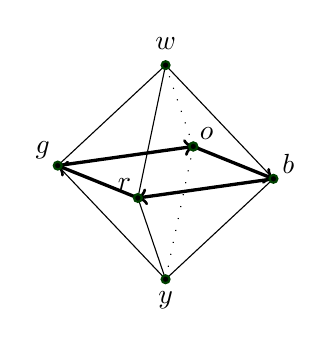
\begin{tikzpicture}%
  [x={(-0.860769cm, -0.121512cm)},
  y={(0.508996cm, -0.205391cm)},
  z={(-0.000053cm, 0.971107cm)},
  scale=1,
  eqback/.style={->, very thick},
  back/.style={loosely dotted, thin},
  eqedge/.style={->, very thick},
  edge/.style={black, thin},
  facet/.style={fill=blue!95!black,fill opacity=0.0},
  vertex/.style={inner sep=1pt,circle,draw=green!25!black,fill=black,thick}]
\coordinate (-1, -1, 0) at (-1, -1, 0);
\coordinate (-1, 1, 0) at (-1, 1, 0);
\coordinate (0, 0, -1) at (0, 0, -1);
\coordinate (0, 0, 1) at (0, 0, 1);
\coordinate (1, -1, 0) at (1, -1, 0);
\coordinate (1, 1, 0) at (1, 1, 0);
%% Drawing edges in the back
%%
\draw[edge,eqback] (-1, -1, 0) -- (-1, 1, 0);
\draw[edge,back] (-1, -1, 0) -- (0, 0, -1.4);
\draw[edge,back] (-1, -1, 0) -- (0, 0, 1.4);
\draw[edge,eqback] (1, -1, 0) -- (-1, -1, 0);
%% Drawing vertices in the back
%%
\node[vertex] at (-1, -1, 0)     {};
%% Drawing the facets
%%
\fill[facet] (1, 1, 0) -- (0, 0, -1.4) -- (1, -1, 0) -- cycle {};
\fill[facet] (1, 1, 0) -- (0, 0, 1.4) -- (1, -1, 0) -- cycle {};
\fill[facet] (1, 1, 0) -- (-1, 1, 0) -- (0, 0, 1.4) -- cycle {};
\fill[facet] (1, 1, 0) -- (-1, 1, 0) -- (0, 0, -1.4) -- cycle {};
%% Drawing edges in the front
%%
\draw[edge] (-1, 1, 0) -- (0, 0, -1.4);
\draw[edge] (-1, 1, 0) -- (0, 0, 1.4);
\draw[eqedge] (-1, 1, 0) -- (1, 1, 0);
\draw[edge] (0, 0, -1.4) -- (1, -1, 0);
\draw[edge] (0, 0, -1.4) -- (1, 1, 0);
\draw[edge] (0, 0, 1.4) -- (1, -1, 0);
\draw[edge] (0, 0, 1.4) -- (1, 1, 0);
\draw[eqedge] (1, 1, 0) -- (1, -1, 0);
%% Drawing the vertices in the front
%%
\begin{scope}[nodes=vertex]
\node[label=above right:\( b \)] at (-1, 1, 0)     {};
\node[label=below:\( y \)] at (0, 0, -1.4)     {};
\node[label=above:\( w \)] at (0, 0, 1.4)     {};
\node[label=above left:\( g \)] at (1, -1, 0)     {};
\node[label=above left:\( r \)] at (1, 1, 0)     {};
\node[label=above right:\( o \)] at (-1, -1, 0)     {};
\end{scope}
\end{tikzpicture}

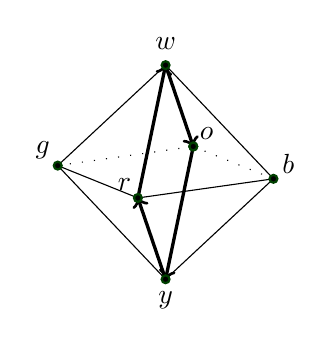
\begin{tikzpicture}%
  [x={(-0.860769cm, -0.121512cm)},
  y={(0.508996cm, -0.205391cm)},
  z={(-0.000053cm, 0.971107cm)},
  scale=1,
  eqback/.style={->, very thick},
  back/.style={loosely dotted, thin},
  eqedge/.style={->, very thick},
  edge/.style={black, thin},
  facet/.style={fill=blue!95!black,fill opacity=0.0},
  vertex/.style={inner sep=1pt,circle,draw=green!25!black,fill=black,thick}]
\coordinate (-1, -1, 0) at (-1, -1, 0);
\coordinate (-1, 1, 0) at (-1, 1, 0);
\coordinate (0, 0, -1) at (0, 0, -1);
\coordinate (0, 0, 1) at (0, 0, 1);
\coordinate (1, -1, 0) at (1, -1, 0);
\coordinate (1, 1, 0) at (1, 1, 0);
%% Drawing edges in the back
%%
\draw[edge,back] (-1, -1, 0) -- (-1, 1, 0);
\draw[edge,eqback] (-1, -1, 0) -- (0, 0, -1.4);
\draw[edge,eqback] (0, 0, 1.4) -- (-1, -1, 0);
\draw[edge,back] (1, -1, 0) -- (-1, -1, 0);
%% Drawing vertices in the back
%%
\node[vertex] at (-1, -1, 0)     {};
%% Drawing the facets
%%
\fill[facet] (1, 1, 0) -- (0, 0, -1.4) -- (1, -1, 0) -- cycle {};
\fill[facet] (1, 1, 0) -- (0, 0, 1.4) -- (1, -1, 0) -- cycle {};
\fill[facet] (1, 1, 0) -- (-1, 1, 0) -- (0, 0, 1.4) -- cycle {};
\fill[facet] (1, 1, 0) -- (-1, 1, 0) -- (0, 0, -1.4) -- cycle {};
%% Drawing edges in the front
%%
\draw[edge] (-1, 1, 0) -- (0, 0, -1.4);
\draw[edge] (-1, 1, 0) -- (0, 0, 1.4);
\draw[edge] (-1, 1, 0) -- (1, 1, 0);
\draw[edge] (0, 0, -1.4) -- (1, -1, 0);
\draw[eqedge] (0, 0, -1.4) -- (1, 1, 0);
\draw[edge] (0, 0, 1.4) -- (1, -1, 0);
\draw[eqedge] (1, 1, 0) -- (0, 0, 1.4) ;
\draw[edge] (1, 1, 0) -- (1, -1, 0);
%% Drawing the vertices in the front
%%
\begin{scope}[nodes=vertex]
\node[label=above right:\( b \)] at (-1, 1, 0)     {};
\node[label=below:\( y \)] at (0, 0, -1.4)     {};
\node[label=above:\( w \)] at (0, 0, 1.4)     {};
\node[label=above left:\( g \)] at (1, -1, 0)     {};
\node[label=above left:\( r \)] at (1, 1, 0)     {};
\node[label=above right:\( o \)] at (-1, -1, 0)     {};
\end{scope}
\end{tikzpicture}

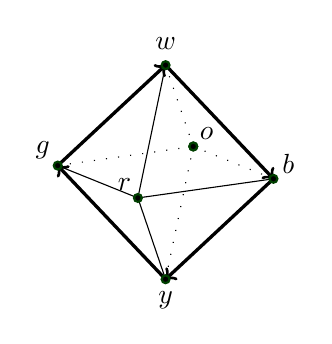
\begin{tikzpicture}%
  [x={(-0.860769cm, -0.121512cm)},
  y={(0.508996cm, -0.205391cm)},
  z={(-0.000053cm, 0.971107cm)},
  scale=1,
  eqback/.style={->, very thick},
  back/.style={loosely dotted, thin},
  eqedge/.style={->, very thick},
  edge/.style={black, thin},
  facet/.style={fill=blue!95!black,fill opacity=0.0},
  vertex/.style={inner sep=1pt,circle,draw=green!25!black,fill=black,thick}]
\coordinate (-1, -1, 0) at (-1, -1, 0);
\coordinate (-1, 1, 0) at (-1, 1, 0);
\coordinate (0, 0, -1) at (0, 0, -1);
\coordinate (0, 0, 1) at (0, 0, 1);
\coordinate (1, -1, 0) at (1, -1, 0);
\coordinate (1, 1, 0) at (1, 1, 0);
%% Drawing edges in the back
%%
\draw[edge,back] (-1, -1, 0) -- (-1, 1, 0);
\draw[edge,back] (-1, -1, 0) -- (0, 0, -1.4);
\draw[edge,back] (-1, -1, 0) -- (0, 0, 1.4);
\draw[edge,back] (1, -1, 0) -- (-1, -1, 0);
%% Drawing vertices in the back
%%
\node[vertex] at (-1, -1, 0)     {};
%% Drawing the facets
%%
\fill[facet] (1, 1, 0) -- (0, 0, -1.4) -- (1, -1, 0) -- cycle {};
\fill[facet] (1, 1, 0) -- (0, 0, 1.4) -- (1, -1, 0) -- cycle {};
\fill[facet] (1, 1, 0) -- (-1, 1, 0) -- (0, 0, 1.4) -- cycle {};
\fill[facet] (1, 1, 0) -- (-1, 1, 0) -- (0, 0, -1.4) -- cycle {};
%% Drawing edges in the front
%%
\draw[eqedge] (-1, 1, 0) -- (0, 0, -1.4);
\draw[eqedge] (0, 0, 1.4) -- (-1, 1, 0);
\draw[edge] (-1, 1, 0) -- (1, 1, 0);
\draw[eqedge] (0, 0, -1.4) -- (1, -1, 0);
\draw[edge] (0, 0, -1.4) -- (1, 1, 0);
\draw[eqedge] (1, -1, 0) -- (0, 0, 1.4);
\draw[edge] (0, 0, 1.4) -- (1, 1, 0);
\draw[edge] (1, 1, 0) -- (1, -1, 0);
%% Drawing the vertices in the front
%%
\begin{scope}[nodes=vertex]
\node[label=above right:\( b \)] at (-1, 1, 0)     {};
\node[label=below:\( y \)] at (0, 0, -1.4)     {};
\node[label=above:\( w \)] at (0, 0, 1.4)     {};
\node[label=above left:\( g \)] at (1, -1, 0)     {};
\node[label=above left:\( r \)] at (1, 1, 0)     {};
\node[label=above right:\( o \)] at (-1, -1, 0)     {};
\end{scope}
\end{tikzpicture}
\caption{The equators for \( w, b, r \).}
\end{figure}
\caption{\( \link \) for the vertices \( w, b\) and \( r \).}
\label{fig:triangle_of_equators}
\end{figure}

To extend \( T_0 \) to a function \( T_1 \) on the 1-skeleton we have complete freedom. Defining a map by induction makes clear that the action on paths is its own structure. Two functions on the octahedron could agree on points but differ on edges. We are going to identify this 1-dimensional freedom with a connection:

Continuing the example, we will do something ``tangent bundley'', imagining how \( T_1 \) changes as we slide from point to point in the embedding shown in the figures. Sliding from \( w \) to \( b \) and tipping the link as we go, we see \( r\mapsto r \) and \( o\mapsto o \) because those lie on the axis of rotation. Then \( g\mapsto w \) and \( b\mapsto y \). 

\begin{mydef}
Define \( T_1:\oo_1\to\EMzo \) on just the 1-skeleton by extending \( T_0 \) as follows:
Transport away from \( w \):
\begin{itemize}
\item \( T_1(wb):[b, r, g, o]\mapsto [y, r, w, o] \) (\( r, o \) fixed)
\item \( T_1(wr):[b, r, g, o]\mapsto [b, y, g, w] \) (\( b, g \) fixed)
\item \( T_1(wg):[b, r, g, o]\mapsto [w, r, y, o] \)
\item \( T_1(wo):[b, r, g, o]\mapsto [b, w, g, y] \)
\end{itemize}
Transport away from \( y \):
\begin{itemize}
\item \( T_1(yb):[b, o, g, r]\mapsto [w, o, y, r] \)
\item \( T_1(yr):[b, o, g, r]\mapsto [b, y, g, w] \)
\item \( T_1(yg):[b, o, g, r]\mapsto [y, o, w, r] \)
\item \( T_1(yo):[b, o, g, r]\mapsto [b, w, g, y] \)
\end{itemize}
Transport along the equator:
\begin{itemize}
\item \( T_1(br):[w, o, y, r]\mapsto [w, b, y, g] \) 
\item \( T_1(rg):[w, b, y, g]\mapsto [w, r, y, o] \)
\item \( T_1(go):[w, r, y, o]\mapsto [w, g, y, b] \)
\item \( T_1(ob):[w, g, y, b]\mapsto [w, o, y, r] \)
\end{itemize}
\end{mydef}

It's very important to be able to visualize what \( T_1 \) does to triangular paths such as \( wb\cdot br\cdot rw \) (which circulates around the boundary of face \( wbr \)). You can see it if you imagine Figure~\ref{fig:triangle_of_equators} as the frames of a short movie. Or you can place your palm over the top of a cube and note where your fingers are pointing, then slide your hand to an equatorial face, then along the equator, then back to the top. The answer is: you come back rotated clockwise by a quarter-turn. 

\begin{mydef}
\label{def:octahedron_holonomy}
The map \( R:C_4\to C_4 \) rotates by one quarter turn, one ``click":
\begin{multicols}{2}
\begin{itemize}
\item \( R(c_1) = c_2 \)
\item \( R(c_2) = c_3 \)
\item \( R(c_3) = c_4 \)
\item \( R(c_4) = c_1 \)
\item \( R(c_1c_2) = c_2c_3 \)
\item \( R(c_2c_3) = c_3c_4 \)
\item \( R(c_3c_4) = c_4c_1 \)
\item \( R(c_4c_1) = c_1c_2 \)
\end{itemize}
\end{multicols}
\end{mydef}

Note by univalence the equivalence \( R \) gives a loop in the universe, a term of \( C_4=_{\EMzo}C_4 \).

Now let's extend \( T_1 \) to all of \( \oo \) by providing values for the eight faces. The face \( wbr \) is a path from \( \refl_w \) to the concatenation \( wb\cdot br\cdot rw \), and so the image of \( wbr \) under the extended version of \( T_1 \) must be a homotopy from \( \refl_{T_1(w)} \) to \( T_1(wb\cdot br\cdot rw) \). Here \emph{there is no additional freedom}.

\begin{mydef}
\label{def:octahedron_curvature}
Define \( T_2:\oo\to\EMzo \) by extending \( T_1 \) to the faces as follows:
\begin{multicols}{2}
\begin{itemize}
\item \( T_2(wbr)=H_R \) 
\item \( T_2(wrg)=H_R \)
\item \( T_2(wgo)=H_R \)
\item \( T_2(ybo)=H_R \)
\item \( T_2(yrb)=H_R \) 
\item \( T_2(ygr)=H_R \)
\item \( T_2(yog)=H_R \)
\item \( T_2(ybo)=H_R \)
\end{itemize}
\end{multicols}
where \( H_R:R=\refl_{C_4} \) is the obvious homotopy given by composition with \( R^{-1} \). Passing through univalence we get a 2-path between \( R \) and \( \refl \) in the loop space \( C_4=_{\EMzo}C_4 \).
\end{mydef}

\subsection{Existence of connections}

How confident can we be that we can always define a connection on an arbitrary combinatorial manifold? Two things make the octahedron example special: the link is a 4-gon at every vertex, and every edge extends to a symmetry of the entire octahedron, embedded in 3-dimensional space. This imposed a coherence on the interactions of all the choices we made for the connection, which we can worry may not exist for more complex combinatorial data.

We know as a fact outside of HoTT that any combinatorial surface that has been realized as a triangulated surface embedded in 3-dimensional euclidean space can inherit the parallel transport entailed in the embedding. We could then approximate that data to arbitrary precision with enough subdivision of the fibers of \( T \).

What would a proof inside of HoTT look like? We will leave this as an open question.


\clearpage
\section{Vector fields}

If \( T:\mm\to\EMzo \) is a bundle of mere circles, then a vector field should consist of, in part, a choice of a point in each fiber:

\begin{mydef}
Let \( \mm:\combmfdt \) be a combinatorial manifold. A \defemph{vector field \( X \) on \( \mm \)} is a section of \( P \) on the 1-skeleton of \( \mm \), i.e. a term \( X:\pit{x:\mm_1}T(x) \).
\end{mydef}
\begin{center}
% https://q.uiver.app/#q=WzAsNCxbMCwyLCJcXG1hdGhiYntNfV8xIl0sWzIsMiwiXFxtYXRocm17RU19KFxcbWF0aGJie1p9LDEpIl0sWzIsMCwiXFxtYXRocm17RU19X1xcYnVsbGV0KFxcbWF0aGJie1p9LDEpIl0sWzAsMCwiUFxcc3RhY2tyZWx7XFxtYXRocm17ZGVmfX09e1xcc3VtX3tDOlRcXG1hdGhiYntNfV8xfUN9Il0sWzAsMSwiVCJdLFsyLDEsIlxcbWF0aHJte3ByfV8xIl0sWzMsMCwiXFxtYXRocm17cHJ9XzEiLDAseyJjdXJ2ZSI6LTF9XSxbMywyLCJcXG92ZXJsaW5le1R9Il0sWzAsMywie1g6XFxwcm9kX3t4OlxcbWF0aGJie019XzF9VHh9IiwwLHsiY3VydmUiOi0xfV0sWzAsMiwiVF9cXGJ1bGxldCJdLFszLDEsIiIsMCx7InN0eWxlIjp7Im5hbWUiOiJjb3JuZXIifX1dXQ==
\begin{tikzcd}
  {P\stackrel{\mathrm{def}}={\sum_{C:T\mathbb{M}_1}C}} && {\mathrm{EM}_\bullet(\mathbb{Z},1)} \\
  \\
  {\mathbb{M}_1} && {\mathrm{EM}(\mathbb{Z},1).}
  \arrow["{\overline{T}}", from=1-1, to=1-3]
  \arrow["{\mathrm{pr}_1}", curve={height=-6pt}, from=1-1, to=3-1]
  \arrow["\lrcorner"{anchor=center, pos=0.125}, draw=none, from=1-1, to=3-3]
  \arrow["{\mathrm{pr}_1}", from=1-3, to=3-3]
  \arrow["{{X:\prod_{x:\mathbb{M}_1}Tx}}", curve={height=-6pt}, from=3-1, to=1-1]
  \arrow["{(T,X)}", from=3-1, to=1-3]
  \arrow["T", from=3-1, to=3-3]
\end{tikzcd}\end{center}


On 1-paths \( p:x=_{\mm_1}y \) \( X \) assigns a choice of pathover \( \pi:\tr(p)(x)=_{Ty}y \), which can also be thought of as a proof of pointedness of the transport map \( \tr(p) \).

The goal now is to recompute the total curvature in the context of some vector field \( X \) and obtain three values:
\begin{enumerate}
\item \todo{Define these systematically}The total curvature, e.g. in the case of \( \oo \) the value \( R^8 \).
\item The total winding of \( X \), which will take the proof of pointedness around all faces in the domain of \( X \). Being a loop in a circle, this is an integer.
\item A pointed version of curvature, which couples the winding of \( X \) to the transport, which is a total function, and which produces a contractible pointed map, i.e. 0.
\end{enumerate}

Once we have these, we will unpack how they provide a proof in HoTT of the Poincaré-Hopf theorem and the Gauss-Bonnet theorem.

\subsection{Index of a vector field: subtracting curvature}

Index should be an integer that computes a winding number ``of the vector field'' around a zero. Classically this is done in a local trivialization around a zero of the vector field, with a canonical flat connection associated to the trivialization (an isomorphism with a product bundle). We should therefore first look for a loop in one of our pointed fibers \( (Tm, Xm) \). Let \( \pi_1,\ldots,\pi_k:L\to\mm \) be a face enumerator with basepoint \( m:\mm \) (Definition~\ref{def:face_enumerator}) and consider the loop \( \ell\defeq\ell_{L,1} \).

\( T\ell:Tm=Tm \) is the holonomy isomporphism of the loop, and it has flatness structure \( H\ell:T\ell=\id_m \). The vector field assigns a dependent path over the loop (a \emph{loopover}) \( X\ell:T\ell(Xm)=Xm \) which is not a closed loop in general. (Remember, this is the whole point of curvature: transporting around a loop does not produce a \emph{pointed} isomorphism of the fiber.)

But notice that the flatness structure tells us exactly how to close the loopover and produce an honest loop in \( (Tm,Xm) \), namely by evaluating \( H\ell \) at \( Xm \), giving \( H\ell(Xm):T\ell(Xm)=Xm \), which is of the same type as \( X\ell \). Forming the concatenation \( X\ell\cdot H\ell(Xm)^{-1}:Xm=Xm \) gives a term in the loop space \( \Omega_{Xm}(Tm)\simeq\zz \). Conceptually, we have asked how much the vector field swirls as it moves around the loop \emph{not counting any swirl of the parallel transport}. The concatenation \( -\cdot H\ell(Xm)^{-1} \) is a subtraction of the effect of curvature.

We have constructed a map \( \Omega_m(\mm)\to \Omega_{Xm}(Tm)\):
\begin{mydef}
The \defemph{index} \( \mathscr{I}_X:\Omega_m(\mm)\to \Omega_{Xm}(Tm) \) is the map \( \ell\mapsto X\ell\cdot H\ell(Xm)^{-1}:Xm=Xm\).
\end{mydef}

\begin{mydef}
The \defemph{total index} of \( X \) is \( \mathscr{I}_X(\ell_{L,1}\cdot\cdots\cdot\ell_{L,k}) \).
\end{mydef}

\subsection{Equality of total index and total curvature}

\begin{comment}
Here we are inspired by the classical proof of Hopf\cite{hopf}, presented in detail in Needham\cite{needham}.

\begin{mydef}
\label{def:enumeration}
An \defemph{enumeration} of a principal bundle with connection and vector field on a higher combinatorial manifold consists of the following data:
\begin{itemize}
\item a family \( T:\mm\to\Kzt \) on some higher combinatorial manifold
\item a nonvanishing vector field \( X:\mm\setminus Z\to P \) with isolated zeros \( Z \)
\item a total face of the replacement \( \mm_Z \) (Definition~\ref{def:totalface}), that is 
\begin{itemize}
\item a basepoint \( a:\mm_Z \) 
\item a term \( f_{\mm_Z}:\refl_a=\refl_a \) given by
\begin{itemize}
\item an ordering of the face constructors \( \{f_i\} \), with the sub-list of faces denoted \( \{f_{zk}\} \) refers to the replacement faces at the zeros
\item a vertex \( v_i \) in each face
\item terms \( a=v_i \) for each face
\end{itemize}
\end{itemize}
\end{itemize}
\end{mydef}

\begin{mynote}
An enumeration let us work both with \( \mm\setminus Z \) where the vector field is nonvanishing, while also having access to the disks that are missing from \( \mm\setminus Z \).
\end{mynote}

\begin{mylemma}
The sub-list of faces \( \{f_i\}-\{f_{zk}\} \) obtained by skipping the replacement faces at the zeros, is an ordering of face constructors for \( \mm\setminus Z \).
\end{mylemma}\begin{proof}
The algorithm that visits each face in order always starts and ends at \( a \) and so we can skip any faces we wish, to obtain an ordering of face constructors for the remaining union of faces.
\end{proof}

Note that on \( \mm\setminus Z \) the vector field \( X \) trivializes the bundle by mapping into the contractible type of pointed types over \( \Kzt \). So \( X\simeq Y:\mm\setminus Z\to (Ta,a) \), the fixed pointed circle in the fiber of the basepoint \( a \). 

\begin{mylemma}
The degree of \( Y \) is minus the total index of \( X \).
\end{mylemma}\begin{proof}
The ordering of faces \( \{f_i\}-\{f_{zk}\} \) provides an ordering of all the edges, say \( \{e_l\} \). Each edge appears an even number of times in this list, traversed in opposite directions, except those bounding a replacement face. These replacement-bounding edges are traversed an odd number of times and can be concatenated to traverse the boundary counterclockwise. Concatenation of paths in \( S^1 \) is abelian, so  \( Y(\{e_l\}) \) cancels except on the boundary of the replacement faces, which gives a map from the disjoint union of boundary circles to \( Ta \), with each boundary circle traversed in the counterclockwise direction. The orientation gives the minus sign.
\end{proof}

Consider now the total face \( f_{\mm_Z} \) of \( \mm_Z \) and its ordering of faces \( \{f_i\} \). \( Y \) is only defined on some of these faces. We will define a new function on all the \( \{f_i\} \).

\begin{mydef}
The \defemph{coupling map} \( C:\mm_Z\to Ta \) is defined to be \( Y \) on \( \mm\setminus Z \) and on the remaining faces it is defined by \( C(f_i)\defeq\apd(X)(\partial f_i) \) where \( \partial f_i:v_i=v_i \) is the clockwise path around the face starting from the vertex supplied by the data of the total face.
\end{mydef}

Because \( \apd \) uses both transport and the value of the vector field, it couples the connection with the vector field, hence the name. Of course in HoTT this coupling is built into the definition of \( \apd \), so that's another reminder that we aren't straying far from the foundations to find these geometrical concepts. 

The fact that \( C \) is defined on all the faces, by using the value of the vector field only on the 1-skeleton of \( \mm_Z \) where it was always defined, lets us make the final part of the argument.

\begin{mylemma}
\( C:\cup_i\{f_i\}\to Ta \) is equal to a constant map.
\end{mylemma}
\begin{proof}
The data of the total face provides an ordering of all the edges. Each edge appears an even number of times, traversed in opposite directions, including the edges in the replacement faces. Concatenation of paths in the polygon \( Ta \) is abelian, so the paths all cancel.
\end{proof}

\( C \) is similar to \( X \) and \( Y \) except that it is a total function. On any given edge it computes a path, that is, a homotopy from the function \( \tr \) to the function \( X \), which we can call ``the difference between transport and the vector field on that edge.'' We have found a way to add all these homotopies together to get 0. We can call this total ``the difference between the total index and the total curvature.''

Recall now that we made some arbitrary choices in Definition~\ref{def:enumeration} of an enumeration, and hence the function \( C \). But since \( C \) is unconditionally constant, the space of extra data is contractible.

\begin{mycor}
The total index of a vector field with isolated zeros is independent of the vector field.
\end{mycor}

\begin{mycor}
The total curvature is an integer.
\end{mycor}

The last step is to link this value to the Euler characteristic.
\end{comment}

\subsection{Identification with Euler characteristic}

\begin{comment}
Here we only point the way. Combinatorial manifolds are intuitive objects that connect directly to the classical definition of Euler characteristic. We can argue using Morse theory, the study of smooth real-valued functions on smooth manifolds and their singularities. Classically the gradient of a Morse function is a vector field that can be used to decompose the manifold into its \emph{handlebody decomposition}. This would be an excellent story to pursue in future work.

Imagine starting with a classical 2-manifold of genus \( g \) that has been triangulated. Stand it upright with the holes forming a vertical sequence. Now install a vector field that points downward whenever possible. This vector field will have a zero at the top and bottom, and one at the top and bottom of each hole. The top and bottom will have zeros of (classical) index 1, and zeros in the holes will have index --1. We include some sketches in the case of a torus (Figure~\ref{fig:torus_morse_skel}). This illustrates how we obtain the formula for genus \( g \): \( \chi(M)=2-2g \). If we choose the triangulation so that the zeros are at vertices, we should be able to import that data into \( \combmfdt \) and reproduce the computation using the tools in this note.

\begin{figure}[htbp]
\centering
% https://q.uiver.app/#q=WzAsOCxbMCwwLCJcXGJ1bGxldCJdLFswLDEsIlxcYnVsbGV0Il0sWzAsMiwiXFxidWxsZXQiXSxbMCwzLCJcXGJ1bGxldCJdLFsxLDAsIlxcbWF0aHJte3RvcH0iXSxbMSwxLCJcXG1hdGhybXt1cHBlclxcIGhvbGV9Il0sWzEsMiwiXFxtYXRocm17bG93ZXJcXCBob2xlfSJdLFsxLDMsIlxcbWF0aHJte2JvdHRvbX0iXSxbMCwxLCIiLDIseyJjdXJ2ZSI6LTEsInN0eWxlIjp7ImJvZHkiOnsibmFtZSI6ImRhc2hlZCJ9fX1dLFswLDEsIiIsMCx7ImN1cnZlIjoxLCJzdHlsZSI6eyJib2R5Ijp7Im5hbWUiOiJkYXNoZWQifX19XSxbMiwzLCIiLDAseyJjdXJ2ZSI6LTEsInN0eWxlIjp7ImJvZHkiOnsibmFtZSI6ImRhc2hlZCJ9fX1dLFsyLDMsIiIsMix7ImN1cnZlIjoxLCJzdHlsZSI6eyJib2R5Ijp7Im5hbWUiOiJkYXNoZWQifX19XSxbMCwzLCIiLDEseyJjdXJ2ZSI6LTV9XSxbMCwzLCIiLDEseyJjdXJ2ZSI6NX1dLFsxLDIsIiIsMSx7ImN1cnZlIjoyfV0sWzEsMiwiIiwxLHsiY3VydmUiOi0yfV1d
\begin{tikzcd}[cramped]
  \bullet & {\mathrm{top}} \\
  \bullet & {\mathrm{upper\ hole}} \\
  \bullet & {\mathrm{lower\ hole}} \\
  \bullet & {\mathrm{bottom}}
  \arrow[curve={height=-6pt}, dashed, from=1-1, to=2-1]
  \arrow[curve={height=6pt}, dashed, from=1-1, to=2-1]
  \arrow[curve={height=-30pt}, from=1-1, to=4-1]
  \arrow[curve={height=30pt}, from=1-1, to=4-1]
  \arrow[curve={height=12pt}, from=2-1, to=3-1]
  \arrow[curve={height=-12pt}, from=2-1, to=3-1]
  \arrow[curve={height=-6pt}, dashed, from=3-1, to=4-1]
  \arrow[curve={height=6pt}, dashed, from=3-1, to=4-1]
\end{tikzcd}
\caption{Schematic of the zeros of the downward flow of a torus.}
\label{fig:torus_morse_skel}
\end{figure}
\end{comment}

\clearpage
\section{The total construction}
\label{sec:totals}
\chcomment[id=Greg]{All new}
We will place holonomy, flatness, and vector fields on the same footing, and combine them. We will prove the equivalance of the total curvature of a tangent bundle, and total index of a vector field. This is the key relationship in proving both the Gauss-Bonnet theorem and the Poincaré-Hopf theorem.

\subsection{Index of the vector field}
Given a polygon cellular type \( C_{n,0}\to C_{n,1}=C_n \), and map \( *_{C_n}:\unit\to\Kzt \) giving it the structure of an \( S^1 \)-torsor, we have the following general fact:
\begin{myprop}
\label{prop:eveq}
Given a pointing \( b:C_n \) the evaluation map \( \ev(b):(C_n=C_n)\to C_n \) is an equivalence.
\end{myprop}
\begin{myproof}
See \cite{buchholtz2023central}.\chcomment[id=Greg]{added citation}
\end{myproof}

Consider the cellular type \( \mm_0\to\mm_1\to\mm \) with point \( m:\mm \). Consider a loop \( \ell:m=_\mm m \) with proof of contractibility \( f:\ell=\refl_m \). For example, we may have a face \( F \) in a combinatorial realization, with \( m \) a vertex of \( F \) and \( \ell=\partial F \) the boundary loop. We have accumulated the following constructions:
\[\begin{aligned}
\tr(\ell)&:Tm=Tm\\
\flat(\ell)&:\tr(\ell)=_{Tm=Tm}\id\\
X(\ell)&:\tr(\ell)(X(m))=_{Tm=Tm}X(m)\\
\end{aligned}\]
which invites us to make use of the equivalence \ref{prop:eveq} to define \( X_E(\ell)\defeq \ev(X(m))^{-1}\circ X(\ell):\tr(\ell)=\id \) (where the subscript \( E \) stands for the extension to all of \( Tm \)) to obtain
\[
\begin{aligned}
\tr(\ell)&:Tm=Tm\\
\flat(\ell)&:\tr(\ell)=_{Tm=Tm}\id\\
X_E(\ell)&:\tr(\ell)=_{Tm=Tm}\id\\
\end{aligned}
\]
These last two can be concatenated to make a loop.
\begin{mydef}
The \defemph{index of the vector field \( X \) around the loop \( \ell \)} is the integer \( I_X(\ell)\defeq\flat(\ell)^{-1}\cdot X_E:\id=_{Tm=Tm}\id \).
\end{mydef}
\begin{mynote}
Classically the index around a loop makes use of a trivialization of the tangent bundle, and does not take place in the presence of a connection. We know from section~\ref{sec:localtriv} that the connection can serve as such a trivialization. Taking that point of view, the formula constitutes the difference between the swirling of the vector field inside the chart, and the twisting of the chart itself. 
\end{mynote}
We now have the following list of ingredients given the loop \( \ell \):
\begin{equation}
\label{eq:face_elements}
\begin{aligned}
\tr(\ell)&:Tm=Tm\\
\flat(\ell)&:\tr(\ell)=_{Tm=Tm}\id\\
X_E(\ell)&:\tr(\ell)=_{Tm=Tm}\id\\
I_X(\ell)&:\id=_{Tm=Tm}\id\\
\end{aligned}
\end{equation}

\subsection{Cancellations}
The next observation is that we can relate the quantities in Equation~\ref{eq:face_elements} at different points around a cellular surface by making use of the automorphism bundle \( \sit{x:\mm}(Tx=Tx) \) and its trivialization \( \tau:\pit{x:M}(Tx=Tx)\xrightarrow[]{\simeq}(Tm=Tm) \) as in Lemma~\ref{lem:gauge_triv}. We will use the action on paths of \( \tau \) to better understand \( \flat \) and \( X_E \) as \emph{angles}.

\begin{mydef}
Consider the contractible type \( \sit{\alpha:Tm=Tm}\alpha=\id \) with the addition law \( (\alpha, p)+(\beta, q) = (\alpha\cdot\beta, p\cdot \alpha(q)) \) where \( \alpha(q):\alpha=\alpha\cdot\beta \) (using concatenation notation instead of function composition). This is a commutative group with identity \( \refl_\id \) which we call the \defemph{type of angles of \( Tm \)}.
\end{mydef}

\begin{mylemma}
\( \tau\circ X \) maps concatenation of paths to the commutative operation \( + \) in the type of angles \( \sit{\alpha:Tm=Tm}\alpha=\id \).
\end{mylemma}
\begin{myproof}
Suppose we have \( p:x=_\mm y \) and \( q:y=_\mm z \). Then \( X(p\cdot q)=\tr(q)(X(p))\cdot X(q) \) which is exactly the operation \( + \) but in the group \( \sit{\alpha:Tz=Tz}\alpha=\id \). We can then transport the result to \( m \) by an arbitrary path.
\end{myproof}

\begin{mycor}
\label{cor:x_cancel}
With \( e, p, \ell \) as in Figure~\ref{fig:lasso}, we have \(\tau(X_E(e\cdot\ell\cdot e^{-1})) = \tau(X_E(\ell))\).
\end{mycor}

So under \( \tau \) we can cancel the contributions to \( X \) from the edge \( e \) after traversing it once in each direction. Meanwhile we have something similar for the transport automorphisms:

\begin{mylemma}
With \( e, p, \ell \) as in Figure~\ref{fig:lasso}, we have \( \tau(\tr(e\cdot\ell\cdot e^{-1}))=\tau(\tr(\ell)) \).
\end{mylemma}
\begin{myproof}
Recall that \( \tau \) conjugates automorphisms by transport along some arbitrary path to \( m \). To transport automorphisms from \( x \) to \( p \), choose a path \( p:m=_\mm x \). Then make the specific choice \( p\cdot e:m=_\mm y \) to transport automorphisms from \( y \) to \( p \). Then \( \tau(\tr(e\cdot\ell\cdot e^{-1})) \) and \( \tau(\tr(\ell)) \) both compute to \( \tr((p\cdot e)\cdot\ell\cdot(p\cdot e)^{-1}) \). 
\end{myproof}

\begin{figure}[h]
\centering
\begin{tikzpicture}[arrow/.style={-{Stealth[scale=1.1]}}]
  \tikzstyle{internal}=[inner sep=0, outer sep=0, line cap=rect]
    \coordinate (V2) at (1, 1.732) {};
    \node[label=below:\( y \)] (y) at (0, 0) {};
    \coordinate (V3) at (2, 0) {};

    \draw (V2) edge["\( \ell \)"] (V3);
    \draw (y) -- (V2);
    \draw[arrow] (V3) -- (y);
    
    \node[label=below:\( m \)] (m) at (-3, 0) {};
    \node[label=below:\( x \)] (x) at (-1.5, 0) {};

    \draw[arrow] (m) edge["\( p\)"] (x);
    \draw[arrow] (x) edge["\( e\)"] (y);
    
    \fill [black] (y) circle (2pt);
    \fill [black] (m) circle (2pt);
    \fill [black] (x) circle (2pt);
\end{tikzpicture}
\caption{Comparing maps on the edge \( e \) at the master point \( m \) with and without traversing \( \ell \).}
\label{fig:lasso}
\end{figure}

\subsection{Total enumeration of faces}
\begin{mydef}
A \defemph{total enumeration of faces} for a combinatorial 2-manifold \( \mm \) with underlying simplicial complex \( M=[M_0, M_1, M_2] \) consists of
\begin{enumerate}
\item A ``master basepoint'' \( m:M_0 \).
\item For each face \( F:M_2 \) with vertices \( \{v_{F,1}, v_{F,2}, v_{F,3}\} \) an enumeration of its vertices \( [v_{F,1}, v_{F,2}, v_{F,3}] \), including the choice of the first vertex in the enumeration as the basepoint of \( F \), which is \defemph{globally compatible} with the choices for the other faces, meaning that when two faces \( F_1,F_2 \) share an edge \( \{v, w\} \), then one of the faces includes the sublist \( [v, w] \) and the other includes \( [w, v] \).
\item An ordering of the faces \( [F_1,\ldots,F_n] \).\chcomment[id=Greg]{Removed the tail of the lasso}
\end{enumerate}
Two enumerations that differ only in the ordering of vertices (2.) are said to have the \defemph{same orientation} if it is true for every face that the two orderings of vertices differ by an even orientation.
\end{mydef}

\begin{mynote}
For such an enumeration to exist the underlying simplicial complex must be \emph{orientable} in a classical sense. We are not going to explore this requirement internally in HoTT, nor prove any relationship between orientability of the set-based complex and orientation in the sense of factoring classifying maps through \( \Kzt\to\EMzo \).
\end{mynote}

\begin{myex}
The octahedron: for \( \oo \) we might choose \( b \) as the master basepoint, as well as the basepoint for four of the faces. For the other four faces we could choose \( g \) as the basepoint. We could choose \( br\cdot rg \) as the path between the basepoints, and we could order the faces like this: \( [bwo, brw, boy, byr, gow, gwr, gry, gyo] \).
\end{myex}

\begin{mydef}
The \defemph{total path} of an enumeration is the list \( \ell_{F_1},\ldots,\ell_{F_n} \) of loops where \( \ell_{F_i}:v_{F_i,1}=v_{F_i,1} \) is the loop around \( F_i \) connecting vertices \( v_{F,1}, v_{F,2}, v_{F,3} \).
\end{mydef}

\begin{mydef}
Using Equation~\ref{eq:face_elements} we can define the \defemph{total curvature}, \defemph{total swirling} and \defemph{total index} of a total path as follows:
\begin{equation}
\label{eq:total_elements}
\begin{aligned}
\flat_\mathrm{tot}&=\tau(\flat(\ell_{F_1}))+\cdots+\tau(\flat(\ell_{F_n}))\\
X_\mathrm{tot}&=\tau(X(\ell_{F_1}))+\cdots+\tau(X(\ell_{F_n}))\\
I_\mathrm{tot}&=\flat_\mathrm{tot}^{-1}\cdot X_\mathrm{tot}
\end{aligned}
\end{equation}
where the sums are taken in the group of angles \( \sit{\alpha:Tm=Tm}\alpha=\id \).
\end{mydef}

\begin{mylemma}
\label{lem:edges_cancel}
The total path of an enumeration visits each edge an even number of times, equally in each direction.
\end{mylemma}

\begin{mythm}
\( \tau(X(\ell_{F_1}))\cdots\tau(X(\ell_{F_n}))=\refl \) in \( \sit{\alpha:Tm=Tm}\alpha=\id \). 
\end{mythm}
\begin{myproof}
Immediate from Lemma~\ref{lem:edges_cancel} and Corollary~\ref{cor:x_cancel}.
\end{myproof}

\begin{mycor}
The total index is equal to the opposite of the total curvature. The total curvature is an integer.
\end{mycor}

\subsection{Total curvature and index on the sphere}

\subsection{Future directions}
Euler characteristic. Chern-Weil theory. Atiyah bundle. Space of connections is contractible. Formalization.

The results of this note can be extended in many directions. There are higher-dimensional generalizations of Gauss-Bonnet, including the theory of characteristic classes and Chern-Weil theory (which links characteristic classes to connections and curvature). These would involve working with nonabelian groups like \( SO(n) \) and sphere bundles. Results from gauge theory could be imported into HoTT, as well as results from surgery theory and other topological constructions that may be especially amenable to this discrete setting. Relationships with computer graphics and discrete differential geometry\cite{crane_ddg}\cite{crane_connections} could be explored. Finally, a theory that reintroduces smoothness could allow more formal versions of the analogies explored here. 

\clearpage
\appendix
\section{Appendix: the program ahead}

Euler characteristic. Chern-Weil theory. Atiyah bundle. Space of connections is contractible. Formalization.

The results of this note can be extended in many directions. There are higher-dimensional generalizations of Gauss-Bonnet, including the theory of characteristic classes and Chern-Weil theory (which links characteristic classes to connections and curvature). These would involve working with nonabelian groups like \( SO(n) \) and sphere bundles. Results from gauge theory could be imported into HoTT, as well as results from surgery theory and other topological constructions that may be especially amenable to this discrete setting. Relationships with computer graphics and discrete differential geometry\cite{crane_ddg}\cite{crane_connections} could be explored. Finally, a theory that reintroduces smoothness could allow more formal versions of the analogies explored here. 

\subsection{The bundle of automorphisms}
\label{sec:automorphisms}
\begin{mydef}
Suppose we have \( T:M\to\EMzo \) and \( P\defeq\sit{x:M}Tx \). Then we can form the type family \( \Aut T:M\to\uni \) given by \( \Aut T(x)\defeq(Tx=Tx) \). The total space \( \Aut P\defeq\sit{x:M}(Tx=Tx) \), which is a bundle of groups, is called the \defemph{automorphism bundle} or the \defemph{gauge bundle} and sections \( \pit{x:M}(Tx=Tx) \), which are homotopies \( T\sim T \), are called \defemph{automorphisms of \( P \)} or \defemph{gauge transformations}.
\end{mydef}

\clearpage

\bibliography{connections}
\end{document}




